\documentclass[twoside,12pt,draft]{PhDThesis}
\usepackage[numbers,sort&compress]{natbib}
\usepackage{epstopdf}
\usepackage{setspace}
\usepackage{pbox}
\usepackage{bbold}
\usepackage{listings}
\usepackage{fixme/fixme}
\usepackage{multicol}
\usepackage{amssymb}
\fxsetup{theme=color}
% \usepackage[toc]{glossaries}
\definecolor{fxnote}{rgb}{0.8000,0.0000,0.0000}


\definecolor{listinggray}{gray}{0.9}
\definecolor{lbcolor}{rgb}{0.9,0.9,0.9}
\definecolor{orange}{cmyk}{0,0.5,1,0}
\lstset{
	backgroundcolor=\color{lbcolor},
	tabsize=4,
	rulecolor=,
	language=matlab,
        basicstyle=\scriptsize,
        upquote=true,
        aboveskip={1.5\baselineskip},
        columns=fixed,
        showstringspaces=false,
        extendedchars=true,
        breaklines=true,
        prebreak = \raisebox{0ex}[0ex][0ex]{\ensuremath{\hookleftarrow}},
        frame=single,
        showtabs=false,
        showspaces=false,
        showstringspaces=false,
        identifierstyle=\ttfamily,
        keywordstyle=\color[rgb]{0,0,1},
        commentstyle=\color[rgb]{0.133,0.545,0.133},
        stringstyle=\color[rgb]{0.627,0.126,0.941},
}
\renewcommand{\indexname}{test1} 

\sisetup{number-unit-product = \text{ }}
%% information for the pdf file
\hypersetup{
 pdfauthor={Lana Beck},
 pdftitle={The Search for the Standard Model Production of Four Top Quarks},
 pdfsubject={The Search for the Standard Model Production of Four Top Quarks}, 
 pdfkeywords={University of Bristol, thesis, top, quark, four} }

% Print URLs not in Typewriter Font
\def\UrlFont{\rm}

\newcommand{\blankpage}{% new clear page without numbering
 \clearpage{\pagestyle{empty}\cleardoublepage}
}

%% setup for the entire document

% hyphenation for words
\hyphenation{
% one-wo-rd an-other-word
}

% open index file
\ifnotdraft{\makeindex}
% \input{inc/pdefs}
%\newcommand {\fig}[1]{fig.\ \ref{#1}}
\newcommand {\Fig}[1]{Fig.\ \ref{#1}}
%%%%%%%%%%%%%%%%%%%%%%%
% comments 
%%%%%%%%%%%%%%%%%%%%%%%
\ifnotdraftelse{
\newcommand{\comment}[1]{}
}{\newcommand{\comment}[1]{{\em #1}}}
% Alles innerhalb von \Hide{} oder \ignore{} 
% wird von LaTeX komplett ignoriert (wie ein Kommentar)
\newcommand{\Hide}[1]{}
\let\ignore\Hide

\newcommand{\mydot}{~\text{.}}



\newcommand{\calL}{\mathcal{L}}
\newcommand{\cL}{\mathcal{L}}
\newcommand{\twovector}[2]{\begin{pmatrix} #1 \\ #2 \end{pmatrix}}
\newcommand{\one}{\ensuremath{\mathbb{1}}}

\newcommand{\cmsSymbolFace}{\mathrm}

\newcommand{\runone}{Run~1\xspace}
\newcommand{\runtwo}{Run~2\xspace}
\newcommand{\lumi}{\ensuremath{\mathcal{L}}\xspace}
\newcommand{\lumiint}{\ensuremath{\mathcal{L}_{\text{int}}}\xspace}
\newcommand {\Et}{$\text{E}_{\text{T}}$\hspace{1mm}}
\newcommand {\Etj}{$\text{E}_{\text{T}}(\text{jet})$\hspace{1mm}}
\newcommand {\mva}{$d_{\text{MVA}}$\hspace{1mm}}
\newcommand {\mvat}{$d^{thresh.}_{\text{MVA}}$\hspace{1mm}}
\newcommand {\etrue}{$\epsilon^{\text{true}}_{\text{QCD}}$\hspace{1mm}}
\newcommand {\est}{$\epsilon^{\text{est.}}_{\text{QCD}}$\hspace{1mm}}

\newcommand{\njetsw}{N\ensuremath{_{\textrm{j}}^{\textrm{W}}}\xspace}
\newcommand{\nMtags}{N\ensuremath{_{\textrm{tags}}^{\textrm{M}}}\xspace}
\newcommand{\nLtags}{N\ensuremath{_{\textrm{tags}}^{\textrm{L}}}\xspace}
\newcommand{\nTtags}{N\ensuremath{_{\textrm{tags}}^{\textrm{T}}}\xspace}
\newcommand{\leadbpt}{p\ensuremath{_{\textrm{T}}^{\textrm{b1}}}\xspace}
\newcommand{\leadleppt}{p\ensuremath{_{\textrm{T}}^{\textrm{l1}}}\xspace}
\newcommand{\htb}{H\ensuremath{_{\textrm{T}}^{\textrm{b}}}\xspace}
\newcommand{\htrat}{H\ensuremath{_{\textrm{T}}^{\textrm{Rat}}}\xspace}
\newcommand{\redhadmass}{M\ensuremath{_{\textrm{RE}}^{\textrm{H}}}\xspace}
\newcommand{\sigmattttsm}{\ensuremath{\sigma_{\tttt}^{SM}}\xspace}

% Physics symbols ...from pdefs
\newcommand{\PT}{\ensuremath{p_{\mathrm{T}}}\xspace}
\newcommand{\pt}{\ensuremath{p_{\mathrm{T}}}\xspace}
\newcommand{\pz}{\ensuremath{p_{\mathrm{z}}}\xspace}
\newcommand {\ptm}{\ensuremath{\pt(\mu)}\xspace}
\newcommand{\ET}{\ensuremath{E_{\mathrm{T}}}\xspace}
\newcommand{\HT}{\ensuremath{H_{\mathrm{T}}}\xspace}
\newcommand{\et}{\ensuremath{E_{\mathrm{T}}}\xspace}
\newcommand{\ETm}{\ensuremath{E_{\mathrm{T}}^{\text{miss}}}\xspace}
\newcommand{\Exm}{\ensuremath{E_{x}^{\text{miss}}}\xspace}
\newcommand{\Eym}{\ensuremath{E_{y}^{\text{miss}}}\xspace}
\newcommand{\vecETm}{\ensuremath{\vec{E}_{\mathrm{T}}^{\text{miss}}}\xspace}
\newcommand{\ETmsquared}{\ensuremath{E_{\mathrm{T}}^{\text{miss } 2}}\xspace}
\newcommand{\MET}{\ETm}
\newcommand{\ETmiss}{\ETm}
\newcommand{\met}{\ETm}
\newcommand{\mex}{\Exm}
\newcommand{\mey}{\Eym}
\newcommand{\vecmet}{\vecETm}
\newcommand{\metsquared}{\ETmsquared}
\newcommand{\ptrat}{\ensuremath{p_{\mathrm{T}}^{Rat}}\xspace}

%particles
\newcommand{\proton}{\ensuremath{\cmsSymbolFace{p}}}
\newcommand{\cPqt}{\ensuremath{\cmsSymbolFace{t}}} % t for t quark
\newcommand{\cPqb}{\ensuremath{\cmsSymbolFace{b}}} % b for b quark
\newcommand{\cPqc}{\ensuremath{\cmsSymbolFace{c}}} % c for c quark
\newcommand{\cPqs}{\ensuremath{\cmsSymbolFace{s}}} % s for s quark
\newcommand{\cPqu}{\ensuremath{\cmsSymbolFace{u}}} % u for u quark
\newcommand{\cPqd}{\ensuremath{\cmsSymbolFace{d}}} % d for d quark
\newcommand{\cPq}{\ensuremath{\cmsSymbolFace{q}}} % generic quark
\newcommand{\cPaqt}{\ensuremath{\overline{\cmsSymbolFace{t}}}} % t for t anti-quark
\newcommand{\cPaqb}{\ensuremath{\overline{\cmsSymbolFace{b}}}} % b for b anti-quark
\newcommand{\cPaqc}{\ensuremath{\overline{\cmsSymbolFace{c}}}} % c for c anti-quark
\newcommand{\cPaqs}{\ensuremath{\overline{\cmsSymbolFace{s}}}} % s for s anti-quark
\newcommand{\cPaqu}{\ensuremath{\overline{\cmsSymbolFace{u}}}} % u for u anti-quark
\newcommand{\cPaqd}{\ensuremath{\overline{\cmsSymbolFace{d}}}} % d for d anti-quark
\newcommand{\cPaq}{\ensuremath{\overline{\cmsSymbolFace{q}}}} % generic anti-quark
\newcommand{\cPg}{\ensuremath{\cmsSymbolFace{g}}} % generic gluon
\newcommand{\cPG}{\ensuremath{\cmsSymbolFace{G}}} % Graviton
\newcommand{\zp}{\ensuremath{\cmsSymbolFace{Z}^\prime}\xspace} % plain Z'
\newcommand{\Z}{\ensuremath{\cmsSymbolFace{Z}}\xspace} % plain Z (no superscript 0)
\newcommand{\ZpJets}{\ensuremath{\Z+\text{jets}}\xspace}
\newcommand{\W}{\ensuremath{\cmsSymbolFace{W}}\xspace}
\newcommand{\WpJets}{\ensuremath{\W+\text{jets}}\xspace}
\newcommand{\VpJets}{\ensuremath{\cmsSymbolFace{V}+\text{jets}}\xspace}
\providecommand{\PH}{\ensuremath{\cmsSymbolFace{H}}\xspace} % plain Higgs
\newcommand{\cPqst}{\ensuremath{\widetilde{\cPqt}}} % t for stop quark
\newcommand{\JPsi}{\ensuremath{\cmsSymbolFace{J}\hspace{-.08em}/\hspace{-.14em}\psi}\xspace} % J/Psi (no mass)
\newcommand{\photon}{\ensuremath{\gamma}\xspace} % plain Z (no superscript 0)
\newcommand{\njets}{N\ensuremath{_{\textrm{jets}}}\xspace}
\newcommand{\nbtags}{N\ensuremath{_{\textrm{btags}}}\xspace}

\newcommand{\Wplus}{\ensuremath{{\cmsSymbolFace{W}}^{+}}\xspace}
\newcommand{\Wminus}{\ensuremath{{\cmsSymbolFace{W}}^{-}}\xspace}
\newcommand{\bbbar}{\ensuremath{\cPqb\cPaqb}\xspace}
\newcommand{\llbar}{\ensuremath{\cmsSymbolFace{l}\overline{\cmsSymbolFace{l}}}\xspace}

\newcommand{\ttbar}{\cPqt\cPaqt\xspace} % t-tbar
\newcommand{\qqbar}{\cPq\cPaq\xspace} % t-tbar
\newcommand{\tttt}{\cPqt\cPaqt\cPqt\cPaqt\xspace}
\newcommand{\ttbb}{\cPqt\cPaqt\cPqb\cPaqb\xspace}
\newcommand{\ttcc}{\cPqt\cPaqt\cPqc\cPaqc\xspace}
\newcommand{\ttll}{\cPqt\cPaqt\textrm{ll}\xspace}

\newcommand{\sigmatttt}{ \ensuremath{\sigma_{{\cPqt\cPaqt\cPqt\cPaqt\xspace}}} }
\newcommand{\sigmattttSM}{ \ensuremath{\sigma_{{\cPqt\cPaqt\cPqt\cPaqt\xspace}}^{SM} } }
\newcommand{\signalstrength}{ \ensuremath{ \frac{ \sigma_{{\cPqt\cPaqt\cPqt\cPaqt\xspace}}  }{\sigma_{{\cPqt\cPaqt\cPqt\cPaqt\xspace}}^{SM}}  } }
\newcommand{\sigmattbb}{\ensuremath{\sigma_{{\cPqt\cPaqt\cPqb\cPaqb\xspace}} } }
\newcommand{\heavyflavour}{ \ensuremath{ \frac{ \sigma_{{\cPqt\cPaqt\cPqb\cPaqb\xspace}}  }{\sigma_{{\cPqt\cPaqt \textrm{jj} \xspace}}}  } }
\newcommand{\heavyflavourone}{ \ensuremath{ \sigma_{\cPqt\cPaqt\cPqb\cPaqb\xspace}}   } 
\newcommand{\heavyflavourtwo}{ \ensuremath{ \sigma_{\cPqt\cPaqt \textrm{jj} \xspace}}  }


\newcommand{\sigttbar}{\ensuremath{\sigma_{\ttbar}}}
%from pdefs END
\newcommand{\tquark}{\ensuremath{\cPqt\text{-quark}}\xspace}
\newcommand{\tquarks}{\ensuremath{\cPqt\text{-quarks}}\xspace}
\newcommand{\bquark}{\ensuremath{\cPqb\text{-quark}}\xspace}
\newcommand{\bquarks}{\ensuremath{\cPqb\text{-quarks}}\xspace}
\newcommand{\cquark}{\ensuremath{\cPqc\text{-quark}}\xspace}
\newcommand{\cquarks}{\ensuremath{\cPqc\text{-quarks}}\xspace}
%new since ttbar + MET
% \newcommand{\mtt}{m$_{\ttbar}$~}
\newcommand{\mtt}{\ensuremath{m_{\ttbar}}\xspace}
\newcommand{\mttbar}{\mtt}
\newcommand{\qq}{$\mathrm{q}\bar{\mathrm{q}}$~}
\newcommand{\xsect}{cross section\xspace} % with or without a hyphen? Make sure it agrees with the usage in the abstract (above)
\newcommand{\xSect}{Cross section} % with an initial capital, but with or without a hyphen?
\newcommand{\CoM}{centre of mass\xspace}
\newcommand{\Nttbar}{N_{\mathrm{t}\overline{\mathrm{t}}}}
\newcommand{\rec}{\mathrm{rec}}
\newcommand{\gen}{\mathrm{gen}}
\newcommand{\MTW}{\ensuremath{M_T(\W)}\xspace}
\newcommand{\ttH}{\ensuremath{\cmsSymbolFace{t}\overline{\cmsSymbolFace{t}}}\ensuremath{\cmsSymbolFace{H}}\xspace}
\newcommand{\ttW}{\ensuremath{\cmsSymbolFace{t}\overline{\cmsSymbolFace{t}}}\ensuremath{\cmsSymbolFace{W}}\xspace}
\newcommand{\ttZ}{\ensuremath{\cmsSymbolFace{t}\overline{\cmsSymbolFace{t}}}\ensuremath{\cmsSymbolFace{Z}}\xspace}
\newcommand{\ttgam}{\ensuremath{\cmsSymbolFace{t}\overline{\cmsSymbolFace{t}}}\ensuremath{\cmsSymbolFace{\gamma}}\xspace}


%unit abbrevations
\newcommand{\pb}{\pico\barn}
\newcommand{\fb}{\femto\barn\xspace}
\newcommand{\pbinv}{\ensuremath{\text{\pb}^{-1}}\xspace}
\newcommand{\fbinv}{\ensuremath{\text{\fb}^{-1}}\xspace}
\newcommand{\mubinv}{\ensuremath{\text{\micro\barn}^{-1}}\xspace}

%generators from pdefs
\newcommand{\GEANT}{{\textsc{GEANT}}\xspace}
\newcommand{\GEANTfour}{{\textsc{Geant4}}\xspace}
\newcommand{\HERWIG}{{\textsc{HERWIG}}\xspace}
\newcommand{\MADGRAPH}{\textsc{MadGraph}\xspace}
\newcommand{\MLM}{\textsc{MadGraph\_MLM}\xspace}
\newcommand{\MCATNLO} {\textsc{MC@NLO}\xspace}
\newcommand{\aMCATNLO} {\textsc{aMC@NLO}\xspace}
\newcommand{\MCFM} {\textsc{MCFM}\xspace}
\newcommand{\POWHEG} {{\textsc{POWHEG}}\xspace}
\newcommand{\PYTHIA} {{\textsc{PYTHIA}}\xspace}
\newcommand{\PYTHIAsix} {{\textsc{PYTHIA6}}\xspace}
\newcommand{\SHERPA} {{\textsc{SHERPA}}\xspace}
\newcommand{\TAUOLA} {\textsc{TAUOLA}\xspace}
\newcommand{\RAW} {\textsc{RAW}\xspace}
\newcommand{\RECO} {\textsc{RECO}\xspace}
\newcommand{\AOD} {\textsc{AOD}\xspace}
\newcommand{\MGfive} {\textsc{Madgraph5\_aMC@NLO}\xspace}
\newcommand{\FASTJET} {\textsc{FastJet}\xspace}
\newcommand{\MADAN} {\textsc{MadAnalysis}\xspace}
\newcommand{\ROOSTAT} {\textsc{RooStat}\xspace}

%other stuff from pdefs
% \newcommand{\CMSSW} {\ensuremath{\text{\verb+CMSSW}}}
\newcommand{\CMSSW} {\textsc{CMSSW}\xspace}
\newcommand{\ROOT} {\textsc{ROOT}\xspace}
\newcommand {\Lone}{Level-1\xspace}
\newcommand{\Tevatron}{TeVatron\xspace}
\newcommand {\DZERO}{D0\xspace}

\newcommand {\ie}{\mbox{i.e.}\xspace}     %i.e.
\newcommand {\eg}{\mbox{e.g.}\xspace}     %e.g.
\newcommand {\etc}{\mbox{etc.}\xspace}     %etc.
\newcommand {\vs}{\mbox{\sl vs.}\xspace}      %vs.
\newcommand {\mdash}{\ensuremath{\mathrm{-}}} % for use within formulas

\newcommand{\stat}{\ensuremath{\,\text{(stat.)}}\xspace}
\newcommand{\syst}{\ensuremath{\,\text{(syst.)}}\xspace}

\newcommand{\DR}{\ensuremath{\Delta R}\xspace}
\newcommand{\Dphi}{\ensuremath{\Delta \phi}\xspace}
\newcommand{\DPTW}{\ensuremath{\Delta {\phi_{\textrm{T-W}}}}\xspace}
\newcommand{\DPTb}{\ensuremath{\Delta {\phi_{\textrm{T-b}}}}\xspace}
\newcommand{\CSVj}{\ensuremath{{\textrm{CSV}}_{\textrm{j}}}\xspace}

%from pdefs (adding a touch of SIunitx) 
%unit abbrevations
\DeclareSIUnit\micron{\micro\meter}
% \newcommand{\micron}{\micro\meter}%this is causing corrupt NFSS tables
% \renewcommand{\micron}{\ensuremath{\mu}\meter}
% roman face derivative
\newcommand{\dd}[2]{\ensuremath{\frac{\cmsSymbolFace{d} #1}{\cmsSymbolFace{d} #2}}}
\newcommand{\ddinline}[2]{\ensuremath{\cmsSymbolFace{d} #1/\cmsSymbolFace{d} #2}}
\newcommand{\rd}{\ensuremath{\cmsSymbolFace{d}}}
% absolute value
\newcommand{\abs}[1]{\ensuremath{\lvert #1 \rvert}}
\newcommand{\alpS}{\ensuremath{\alpha_S}\xspace}
\newcommand{\alpEM}{\ensuremath{\alpha_{\text{em}}}\xspace}
\newcommand{\kt}{\ensuremath{k_{\mathrm{t}}}\xspace}
\newcommand{\antikt}{\ensuremath{\mathrm{anti}\text{-}k_{\mathrm{t}}}\xspace}
\newcommand{\pc}{\%}

%triggers
\newcommand{\HLTThreeCentralJetNonIso}{HLT-Ele25-CaloIdVT-TrkIdT-TriCentralJet30\xspace}
\newcommand{\HLTThreeCentralJet}{HLT-Ele25-CaloIdVT-CaloIsoT-TrkIdT-TrkIsoT-TriCentralJet30\xspace}
\newcommand{\HLTThreeCentralPFJet}{HLT-Ele25-CaloIdVT-CaloIsoT-TrkIdT-TrkIsoT-TriCentralPFJet30\xspace}

\newcommand{\reliso}{\ensuremath{\text{reliso}}\xspace}
\newcommand{\bjet}{\ensuremath{\text{\cPqb-jet}}\xspace}
\newcommand{\btag}{\ensuremath{\text{\cPqb-tag}}\xspace}
\newcommand{\btags}{\ensuremath{\text{\cPqb-tags}}\xspace}
\newcommand{\btagging}{\ensuremath{\text{\cPqb-tagging}}\xspace}
\newcommand{\btagged}{\ensuremath{\text{\cPqb-tagged}}\xspace}
\newcommand{\pdf}{\ensuremath{\mathrm{pdf}}}
\newcommand{\multijet}{multi-jet\xspace}
\newcommand{\eplusjets}{electron channel}
\newcommand{\muplusjets}{muon channel}

\newcommand{\Niexp}{\ensuremath{N_i^\text{exp}}}
\newcommand{\Niobs}{\ensuremath{N_i^\text{obs}}}
\newcommand{\U}{\ensuremath{\text{U}}}
\newcommand{\SU}{\ensuremath{\text{SU}}}

\newcommand{\HTX}{\ensuremath{{\textrm{HT}}_{\textrm{X}}}\xspace}
\newcommand{\sumjetmassX}{\ensuremath{{\textrm{SumJetMass}}_{\textrm{X}}}\xspace}

\newcommand{\HTb}{\ensuremath{{\textrm{HT}}^{\textrm{b}}}\xspace}
\newcommand{\HTrat}{\ensuremath{{\textrm{H}}_{\textrm{T}}^{\textrm{rat}}}\xspace}

\newcommand{\CLS}{\ensuremath{{\textrm{CL}}_{\textrm{S}}}\xspace}

\hyphenation{brems-strah-lung}
\hyphenation{lep-ton-ic}
\hyphenation{di-lep-ton-ic}

\graphicspath{{images/}}

%%%%%%%%%%%%%%%%%%%%%%%%%%%%%%%%%%%%%%%%%%%%%%
\doublespace
\begin{document}
%roman page numbering for Title page, abstract and index
\pagenumbering{roman}


%titlepage start
\titlehead{%
\large\resizebox{!}{1.2cm}{%
\includegraphics{images/Bris_logo-colour}}%
~~~
\large\resizebox{!}{1.2cm}{%
\includegraphics{images/logo_vub_fullP.pdf}}%
\hfill\raise3.5mm\hbox{School of Physics}
} % end titlehead

\titlefoot{%
\raise3.5mm\hbox{University of Bristol, Vrije Universiteit Brussel}\ 
\hfill\resizebox{!}{1.3cm}{%
\includegraphics*{images/CMS_logo_May2014-eps-converted-to.pdf}}%
}

\begin{titlepage}
%\let\footnotesize\small \let\footnoterule\relax
\begin{center}
\hbox{}
\vfill
{\LARGE\bfseries The Search for the Standard Model Production of Four Top Quarks

\par} 
\vskip 3.5cm
{\Large Lana Beck}\\

\vskip 7cm
A dissertation submitted to the University of Bristol and Vrije Universiteit Brussel in accordance
with the requirements of the degree of PhD in the Faculty of Science,
School of Physics, Bristol and Faculteit Wetenschappen en Bio-ingenieurswetenschappen, Vakgroep Fysica, Brussel.\\[2ex]
Dec 2016\\ [2ex]
\vskip 1.5cm
% \textbf{Lana Beck}\\
\end{center}
\vfill
\end{titlepage}

%\addcontentsline{toc}{chapter}{Cover page}
\label{c:abstract}
\chapter*{Abstract} 
% The results of the search for four top quark production are presented...{
\small{
The Standard Model (SM) of Particle Physics has been incredibly successful and accurate in describing the fundamental particles that make up the world around us and they way they behave. However, we know it is not the ultimate theory of nature as some phenomena remain unexplained. Outstanding questions include what is dark matter, this mysterious material which can be inferred from observations of the universe but has not been directly detected; and where does gravity fit into the picture? These questions motivate our search for physics Beyond the Standard Model (BSM) at the Large Hadron Collider at the CERN research facility. Here we accelerate protons around a 27 km ring and collide them at four experiments located underground. When we collide protons we effectively collide the more fundamental particles within the protons, quarks and gluons.

This thesis focuses on research undertaken at the CMS experiment studying the heaviest quarks, top quarks, which are not found in nature but instead are produced in high-energy experiments. Top quarks are most often produced in pairs, however this thesis focuses on the search for the simultaneous production of four top quarks, which is an incredibly rare process in comparison. A precision measurement of this rare process would be a stringent test on the SM and may give hints of physics beyond the standard model. 
Untangling the signal of four-top-quark production from the overwhelming background of top-quark-pair production in the output of the detector is incredibly difficult. Algorithms, which are often used in developing artificial intelligence, are therefore employed to exploit subtle differences in signatures, greatly increasing the sensitivity.
Results are presented which place tight limits on the rate of four-top-quark production, and projections of the future sensitivity are made including an estimate of when CMS will have sufficient data to definitively observe this process at SM rates. The results allow us to place constraints on properties of hypothesised BSM particles. Here we interpret the results to place constraints on the mass and top quark-coupling of one such particle, the sgluon.}

\clearpage
\chapter*{Samenvatting}
\footnotesize{ Het Standaard Model (SM) van deeltjesfysica is ongelofelijk succesvol en nauwkeurig in het beschrijven van de fundamentele deeltjes in de wereld om ons heen en de manier waarop ze zich gedragen. Maar we weten dat het niet de ultieme natuurkundige theorie is, omdat een aantal verschijnselen onverklaard blijven in het SM. Openstaande vragen zijn: wat is donkere materie, het bestaan van deze mysterieuze substantie kan worden afgeleid uit waarnemingen van het heelal, maar is nog niet rechtstreeks waargenomen; en waar past de zwaartekracht in het plaatje? Deze vragen motiveren onze zoektocht naar de fysica voorbij het Standaard Model (BSM) bij de Large Hadron Collider op het CERN. Hier versnellen we protonen rond een ring van 27 km omtrek. Op vier plaatsen aan de ring liggen ondergrondse experimenten waar de protonen worden gebotst. Wanneer protonen botsen, bestuderen we effectief de werkelijk fundamentele deeltjes in het proton, quarks en gluonen. 
Dit proefschrift richt zich op onderzoek gebruikmakend van de proton-proton botsingen waargenomen door het CMS-experiment. Het zwaarste bekende elementaire deeltje, de top-quark, is niet te vinden in de natuur, maar in plaats daarvan kan worden geproduceerd in de botsingen bij de LHC. Top quarks worden meestal geproduceerd in paren, maar dit proefschrift richt zich op de zoektocht naar de productie van vier top-quark tegelijkertijd, dat is een ongelooflijk zeldzaam proces in vergelijking met paarproductie. Een nauwkeurige meting van deze zeldzame proces zou een strenge test zijn van het SM en kan hints geven of er nieuwe deeltjes worden gemaakt samen die in vier top quarks uiteenvallen. Het identificeren van het signaal van vier top-quark productie in de overweldigende achtergrond van top-quark-paarproductie in de data is een ongelooflijk moeilijke wetenschappelijke uitdaging. Hiervoor worden machine-learning algoritmen toegepast. Op deze wijze kunnen subtiele verschillen tussen de productie van top quark paren en vier top quarks in de botsing worden benut, en dit leidt tot een aanzienlijke verhoging van de gevoeligheid van de data-analyse. 
De resultaten van dit onderzoek plaatsen de meest strakke grenzen aan de werkzame doorsnede voor productie van vier top quarks. De resultaten zijn ook in staat om beperkingen te geven op de eigenschappen van eventuele hypothetische BSM deeltjes. In dit onderzoek worden daarom de resultaten ook ge{\"i}nterpreteerd als een functie van de massa en top quark-koppeling van zo'n hypothetisch nieuw deeltje, het zogenaamde sgluon.}

\normalsize

%\addcontentsline{toc}{chapter}{Abstract}
\chapter*{Acknowledgements} 

Stuff that's supposed to make you emotional..

%\addcontentsline{toc}{chapter}{Acknowledgements}
%% ++++++++++++++++++++++++++++++++++++++++++
%% index
%% ++++++++++++++++++++++++++++++++++++++++++
% {\parskip 0pt\tableofcontents}
\tableofcontents
%\addcontentsline{toc}{chapter}{Table of Contents}
\cleardoublepage
%\listoffigures
%\addcontentsline{toc}{chapter}{List of Figures}
%\blankpage
%\listoftables
%\addcontentsline{toc}{chapter}{List of Tables}
%\blankpage

%change page numbering back to arabic (and start from 1) 
\pagenumbering{arabic}

%% ++++++++++++++++++++++++++++++++++++++++++
%% main part
%% ++++++++++++++++++++++++++++++++++++++++++
\mainmatter

\chapter{Introduction}
\label{c:intro}

The standard model (SM) of particle physics is the currently accepted theory for describing the known fundamental building blocks of the universe. It includes the six quarks and six leptons (and their anti-particles), and the four fundamental forces, electromagnetism, weak force, strong force and gravity. It also includes the Higgs boson that arises from the Brout-Englert-Higgs mechanism, which describes the origin of mass of the quarks, leptons and weak gauge bosons.
It has stood up to rigorous testing at experiments such as at the Deutsches Elektronen-Synchrotron (DESY), the Large Electron Positron collider (LEP) at CERN and the Tevatron at Fermilab. However there are still many unanswered questions about the universe such as how does gravity fit in when it is not described in the SM? What is the dark matter in the universe that affects galaxy rotation curves and causes gravitational lensing where no baryonic matter is present. 
The Large Hadron Collider (LHC) at CERN aims to answers these question by studying the possible signatures of new physics that may arise around the electroweak scale. One of the main goals of the LHC was to find the Higgs boson which was confirmed in July 2012. The precision measurement of SM processes is also still very important as deviations from the SM expectation can give hints about new physics and they are also key background processes which should be well understood so that new physics signals can be found.

The SM process of the production of four top quarks is studied in this thesis. Although this process is predicted by the SM, it is extremely rare and hence it has not yet been possible to measure it. A precision measurement of four top quark production would be an exceptional test of the SM. In addition to this, many models of new physics predict final states which contain four top quarks including supersymmetry, models with extra dimensions, models where the top quark/Higgs boson is a composite particle, or models which contain pair-produced scalar particle which decay into top quark pairs.
Therefore the SM production of four top quarks is both an important background to these new models and the production rate of four top quarks may be enhanced by new physics models.

The thesis is structured as follows: First the background theory of particle physics and top quark physics is discussed in Chapter~\ref{c:theory}. The LHC and particularly the CMS detector are described in Chapter~\ref{c:det}. The reconstruction of physics objects from the detector read-out are given in Chapter~\ref{c:recon}. In Chapter~\ref{c:ana} the general strategy for searching for four top quarks and the analytical and statistical techniques required are described. The search for four top quarks in the single lepton channel in the 2012 dataset collected by the CMS experiment at $\sqrt{s}=8$~TeV is described in Chapter~\ref{c:Run1}. The phenomenological interpretation of the former analysis and another CMS same-sign dilepton analysis in the context of a model of new physics where a sgluon particle is predicted is given in Chapter~\ref{c:pheno}. The search for four top quarks is continued in the 2015 dataset collected by the CMS experiment at $\sqrt{s}=13$~TeV, described in Chapter~\ref{c:Run2}, where enhancements are made to the analysis and additional search channels, opposite-sign and same-sign dilepton are combined with the single lepton channel to produce a more sensitive final result. Finally a summary of the thesis can be found in Chapter~\ref{c:DandC}, including a discussion of the relevance of the analysis in the field of high energy physics and a look towards the future.

The author's personal contributions to the analyses in this thesis include: 
\begin{itemize}
\item In Chapter~\ref{c:Run1}, on the search for four top quarks at $\sqrt{s}=8$~TeV, Sections~\ref{sec:QCDbackground},~\ref{sec:njetcatlimit} and~\ref{studies8}.
\item All of the work in Chapter~\ref{c:pheno}, except on Figure~\ref{fig:sgluonExclusion}, the result from the single lepton channel was not the author's work.
\item In Chapter~\ref{c:Run2}, on the search for four top quarks at $\sqrt{s}=13$~TeV, all sections except for the training of the hadronic top BDT in Section~\ref{sec:topContent13} are the author's work.
\end{itemize}


In this thesis the convention of using natural units, $\hbar = c = 1$, is adopted. 

%\addcontentsline{toc}{chapter}{Introduction}
\chapter{Theory}
\label{c:theory}


\section{Standard Model}

\section{Four top quark production}

\section{BSM models with four top quark signatures}
%\addcontentsline{toc}{chapter}{Theory}
\chapter{The CMS detector and the Large Hadron Collider}
\label{c:det}
This chapter discusses the Large Hadron Collider (LHC) which is located on the Franco-Swiss border near Geneva approximately 100 m undergrounds at the site of the Centre European de Research Nuclear (CERN). It is a 26.7 km long synchrotron particle accelerator with four interaction points where four experiments are located.  My thesis focuses on results from the Compact Muon Solenoid detector described in section~\ref{sec:CMSdet}. The other experiments include ATLAS which is a multi-purpose experiment like CMS, the LHCb detector which focusses on the study of the physics of B mesons and the ALICE detector which is used to study quark-gluon plasmas.

\section{LHC}

The LHC accelerates two beams of protons which circulate in opposite directions \fixme{describe opposite magnetic dipoles}. The protons are sourced from a bottle of hydrogen where a strong electric field is used to rip apart the electrons from the hydrogen atom leaving protons behind. The protons are then accelerated through the linear accelerator LINAC2 before being injected into the Proton Synchrotron Booster (PSB), then into the Proton Synchrotron (PS) followed by the Super Proton Synchrotron (SPS) which is the final accelerator before the protons are injected into the LHC ring. Each accelerator stage boosts the protons to a higher energy, as seen in fig.\fixme{add figure} before they can be injected into the LHC where their final collision energy can be achieved.

\begin{figure}[ht!]
\centering
    \includegraphics[width=0.95\textwidth]{images/LHCacc.jpg}
    \caption{The LHC accelerator complex at CERN}
    \label{fig:LHC acc}
\end{figure}


 The LHC was designed to have a centre of mass collision energy of $\sqrt{s} = 14 \TeV$. However, after an incident 10 days into operation in 2008 which caused damage to the LHC, it was restarted with the lower energy of $\sqrt{s} = 7 \TeV$ in 2011. In 2012 this was increased to $\sqrt{s} = 8 \TeV$ and a dataset with a \fixme*{luminosity}{explain lumi} of $\approx 20 \fbinv$ was recorded. This dataset was used for the analysis in chapter~\ref{c:Run1}. Further details on the run conditions can be found in \fixme{table of lumi, bunches etc.}. In 2013 after the run phase known as \emph{Run 1}, Long Shutdown 1 (LS1) commenced to make upgrades to the LHC and the detectors to allow the machine to run at $\sqrt{s} = 13 \TeV$ for \emph{Run 2}. Run 2 began in March 2015 and results from Run2 are the focus of the analysis in chapter~\ref{c:Run2}.

Run1 saw the great success of the discovery of the Higgs boson, one of the main objections of the LHC. In Run2, the search for new physics continues where precision measurements will test the predictions of the Standard Model.

\section{CMS detector}
\label{sec:CMSdet}

\subsection{Magnetic Solenoid}

\subsection{Tracker}

\subsection{Electromagnetic Calorimeter}

\subsection{Hadronic Calorimeter}

\subsection{Muon Chambers}

\subsection{Trigger}



\subsection{Upgrades for Run II}

% \addcontentsline{toc}{chapter}{Detector}
\chapter{Event Reconstruction}
\label{c:recon}
% In this chapter the software and algorithms used to reconstruct particle physics objects are detailed. The idea is to work backwards from the information obtained from each of the sub-detectors to determine what particles passed through them.\\
% A software framework known as CMSSW has been developed in order to reconstruct the read out from the detector for each event


In chapter~\ref{c:det} each of the sub-detectors in CMS have been described; how particles interact with them and how electrical signals are read-out. The next step is to combine the read-outs from each detector in order to reconstruct the resulting particles from an interesting proton-proton collision. This snapshot of the collision output is known as an \emph{event}. An event will also contain reconstructed particles from other simultaneous uninteresting collisions from the same bunch crossing which is known as \emph{pile up} (PU). Algorithms are used in order to subtract PU particles from the stored event. 
As a particle will usually traverse more than one sub-detector, it is advantageous to combine these outputs in order to reconstruct the particle. This is achieved using the \emph{Particle flow} (PF) algorithm described in section~\ref{sec:PF}. The objects which can be reconstructed using the PF algorithm such as primary vertices, muons, electrons, and jets are discussed in sections~\ref{sec:PVreco},~\ref{sec:muonreco},~\ref{sec:electronreco},~\ref{sec:jetreco} respectively. Further information can be obtained from these reconstructed objects such as how likely a jet is to have originated from a b-quark (section~\ref{sec:btagreco}) and how the presence of neutrinos can be inferred by the imbalance of energy in the transverse plane of the detector (section~\ref{sec:METreco}).  
The information from the detector is processed using a distributed computing infrustruction with the CMSSW software \fixme{reference}.
% This chapter will discuss the main software used to reconstruct events from the detector read-out, CMSSW, and how a worldwide computer farm is used to process data.


% \section{Software}

% To-do:
% CMSSW, grid

\section{Track reconstruction}

\section{Particle flow ~\label{sec:PF}}

The particle flow (PF) algorithm combines information from all sub-detectors, described in section~\ref{c:det}, in order to improve the reconstruction of final state particles such as electrons, muons, photons, neutral hadrons and charged hadrons. The biggest gains come from PF jet reconstruction where the jet-matching efficiency, jet energy resolution and the reconstruction of the jet \pt are improved compared to using calorimeter information only. From this information more complicated objects can be reconstructed as described in the subsequent sections~\ref{CMS-PAS-PFT-10-001}.\\

The first objects reconstructed are PF muons. Each muon identified from the muon chambers is associated to the compatible hits in the tracker. This track is then removed from the collection. Next, a Gaussian-Sum-filter refit is used to extrapolate electron candidate trajectories to the ECAL. Electrons have relatively short tracks due to losing most of their energy by Bremsstrahlung in the tracker material. Tracker and ECAL variables are combined for the final identification of a PF electron after which the track and ecal clusters are removed from the collection.

Charged hadrons are reconstructed from the remaining tracker, ECAL and HCAL deposits where the calorimeter hits are compatible with the tracker hits. Again, these hits are removed from the collection. Neutral hadrons leave no tracks in the tracker but have deposits in the ECAL and HCAL. Photons leave deposits in the ECAL but not the HCAL.

\section{Primary vertices \label{sec:PVreco}}

Primary vertices are the point at which the collision occurred, as opposed the secondary vertices which originate at the decay of subsequest particles coming from the collision. The first step in reconstructing primary vertices is to consider tracks which are consistent with the beam spot and cluster them into candidate vertices, separated along the z direction. Next a 3D fit is made and candidates which are compatible with originating from the beamline are kept.

\section{Muons \label{sec:muonreco}}
The signal muons used in this analysis are selected from the collection of PF muons with the further requirements shown in table~\ref{tab:muon_tight_cuts}.
Relative isolation (\emph{RelIso}), is a measure of how isolated the muons (or electrons) are from surrounding hits in the detector from charged hadrons, neutral hadrons and photon energy. Only charged hadrons which are consistent with the primary vertex are considered in the calculation. As it is not possible to determine whether neutral hadrons are consistent with the primary vertex we can use the fact that the ratio of neutral to charged energy has been measured to be $\approx 0.5$. Hence the neutral hadronic energy coming from the primary vertex can be calculated as seen in Eqn.~\ref{eqn:neutralE}, where $E_{T,sub-leading}^{charged hadronic}$ is the transverse energy from charged hadrons which are associated to a sub-leading primary vertex. This is called the \emph{deltaBeta correction}. The max() function ensures that the corrected neutral hadronic energy is never defined as negative.

\begin{centering}
\begin{equation}
\Sigma E_{T}^{Corrected Neutral Hadronic}  =  max(0, \Sigma E_{T}^{Neutral Hadronic} - 0.5*\Sigma E_{T,sub-leading}^{charged hadronic} )
\label{eqn:neutralE}
\end{equation}
\end{centering}



The RelIso formula with deltaBeta correction can be found in~\ref{eqn:dBRelIso}. It is defined in a cone of $\textrm{R}=0.4$ and scaled by $1\; / \;\pt^{\mu}$ so that lower momemtum muons are required to have less energy from hadrons and photons in the cone to be considered isolated.

\begin{centering}
\begin{equation}
RelIso = \left( \Sigma E_{T}^{charged hadronic} + \Sigma E_{T}^{Corrected Neutral Hadronic} +  \Sigma E_{T}^{Photons} \right) \; / \;   \pt^{\mu}
\label{eqn:dBRelIso}
\end{equation}
\end{centering}

\begin{table}[htpb!]
\footnotesize
\begin{center}
\begin{tabular}{c|c}
\hline
&  Requirements\\
\hline
Is a GlobalMuon and a TrackerMuon & yes \\
\pt (\GeV) $>$ & 26  \\
$\lvert \eta \rvert <$  &  2.1 \\
Number of valid hits in the tracker $>$ & 5 \\
Number of hits in the muon stations $>$ & 0\\
Transverse impact parameter wrt leading primary vertex (cm) $<$ & 0.2\\
dz between leading primary vertex the muon track (cm) $<$ & 0.5 \\
Number of pixel hits $>$ &  0 \\
Normalised $\chi^{2}$ of track $<$ & 10 \\
Number of matched muon stations $>$ & 1\\
Relative Isolation, RelIso, $<$ & 0.15 \\
\hline
\end{tabular}
\caption{The cuts used for the tight muon identification}
\label{tab:muon_tight_cuts}
\end{center}
\end{table}


Loose muons are defined as satisfying the following less strict criteria.
\begin{itemize}
\item Is GlobalMuon or a TrackerMuon
\item  \pt $>$ 10 
\item $\lvert\eta \rvert < 2.5$
\item  RelIso, $<$ 0.25 
\end{itemize}

\section{Electrons \label{sec:electronreco}}
Signal electrons are selected from the collection of PF electrons and are required to pass the criteria for tight electrons given for electrons which are found in the barrel and endcap in table~\ref{tab:electron_tight_cuts}. The RelIso for electrons is defined similarly to muons however the deltaBeta correction is replaced by a rho correction, defined in equation~\ref{eqn:rhoCorr} where EA denotes Effective Area. [EA: derived from the event-specific average pile-up energy density per unit area in the phi-eta plane (rho) and the effective area based on shower shapes that the EGM POG has measured (depends on supercluster eta).]

\begin{centering}
\begin{equation}
rhoCorr = \left( \Sigma E_{T}^{Neutral Hadronic} + \Sigma E_{T}^{Photons} - \rho\times\textrm{EA} \right) 
\label{eqn:rhoCorr}
\end{equation}
\end{centering}


\begin{centering}
\begin{equation}
RelIso = \left( \Sigma E_{T}^{charged hadronic} + rhoCorr \right) \; / \;   \pt^{e}
\label{eqn:dBRelIso}
\end{equation}
\end{centering}

\begin{table}[htpb!]
\footnotesize
\begin{center}
\begin{tabular}{c|c|c|c|c}
\hline
& \multicolumn{2}{c|}{Tight} & \multicolumn{2}{c}{Veto} \\
\cline{2-5}
%&Tight & TIght & Veto & Veto \\
&  Barrel        &   Endcap  &  Barrel        &   Endcap  \\
%&  ($|\eta_{SuCluster}|< 1.4442$)         &   ($1.5660<|\eta_{SuCluster}|<2.5$)  &  ($|\eta_{SuCluster}|< 1.4442$)         &   ($1.5660<|\eta_{SuCluster}|<2.5$)  \\

\hline
full $5\times5 \; \sigma_{I_{\eta}I_{\eta}} < $ & 0.0101 & 0.0279 & 0.0114 & 0.0352\\
$|\Delta \eta_{In}| < $  & 0.00926 & 0.00724  & 0.0152 & 0.0113  \\
$|\Delta \phi_{In}| < $  &  0.0336 & 0.0918 &  0.216 & 0.237  \\
$\frac{h}{E} <$ &0.0597 & 0.0615  &0.181 & 0.116  \\
relIso with rho correction  $\leq$  & 0.0354 & 0.0646& 0.126 & 0.144\\
$\frac{1}{E} - \frac{1}{p} < $ & 0.012 & 0.00999  & 0.207 & 0.174 \\
$|$d$0| < $  & 0.0111 & 0.0351  & 0.0564 & 0.222\\
$|$dz$| < $  & 0.0466 & 0.417 & 0.472 & 0.921\\
expected missing inner hits $\leq$ & 2 & 1 & 2 & 3  \\
pass conversion veto & yes & yes& yes & yes  \\
\hline
\end{tabular}
\caption{The cuts used for the tight and veto electron identification where barrel is $|\eta_{SuCluster}|< 1.4442$ and endcap is  ($1.5660<|\eta_{SuCluster}|<2.5$)}
\label{tab:electron_tight_cuts}
\end{center}
\end{table}


\section{Jets \label{sec:jetreco}}
When partons such as quarks and gluons fragment and hadronise in the detector, predominantly into charged and neutral hadrons, they form showers of particles in approximately the same direction of travel as the original parton. These final state particles can be clustered into what is known as a \emph{jet} using the anti-$\kappa_{\textrm{T}}$ reconstruction algorithm~\cite{Cacciari:2008gp}. For the analyses in this thesis a cone radius of R = 0.4 is used to reconstructed jet objects. Corrections are applied to the jet energy to account for the non-uniform response of the detector in \pt and $\eta$. These are known as the \fixme*{ref and check if different between 8 \& 13}{L1FastJet and L2L3Residual}. The jet energy resolution (JER) is also smeared by 10$\%$ as the resolution is worse in data than in simulation. Loose jet identification critera are applied to suppress fake jets arising from lepton showers. This includes requiring $|\eta|<2.5$, \pt$<30$ and a separation from the nearest loose muon or electron of $\Delta\textrm{R}>0.4$ \fixme{Check R has been defined}.

\section{b-tagging ~\label{sec:btagreco}}
Reconstructing jets gives us the knowledge that the particles emerging from the collision include quarks. Being able to identify which flavour of quark showered in the detector is extremely useful for a wide range of analyses. Particularly for searches for final states containing four top quarks, the ability to identify b-quarks originating from the decay of top quarks is incredibly beneficial in allowing us to suppress backgrounds and for forming discriminating variables between the signal and irreducible backgrounds. 

The particle shower coming from the hadronisation of b-quarks will contain B mesons which travel further in the detector due to having longer decay times than light flavour mesons (u,d,s,g). The \emph{impact parameter} (IP), defined as the distance between the primary vertex and the extrapolated point of closest approach of a track, will be larger for tracks coming from the decay of a B meson. The tracks emerging from this decay will form a secondary vertex. This information is exploited in the Combined Secondary Vertex (CSV) algorithm. The CSV algorithm is used to identify or \emph{tag} jets which originate from b-quarks by assigning a discriminator value between 0 and 1, where larger values are more consistent with b-quark jets. Loose (CSVL), medium (CSVM) and tight (CSVT) working points are defined at values of the discriminator for a given mis-identification rate. For analyses at $\sqrt{s} = 13$~TeV the algorithm was improved and is called Combined Secondary Vertex version 2 algorithm (CSVv2). Working points, selection efficiencies for b-quarks and mis-identification rates are gien in table~\ref{tab:btag} \footnote{This efficiency was measured using the TTJets MLM sample for the medium working point at $\sqrt{13}$ TeV. The CSVv2L and CSVv2T efficiences have been taken from here~\cite{btageff} }.

\begin{table}[htpb!]
\footnotesize
\begin{center}
\begin{tabular}{l|l|c|c|c}
$\sqrt{s}$ (TeV)    & Name   & \multicolumn{1}{l|}{WorkingPoint} & \multicolumn{1}{l|}{Selection Efficiency ($\%$)} & \multicolumn{1}{l}{Mis-identification ($\%$)} \\ \hline
\multirow{3}{*}{8}  & CSVL   & 0.244                             &                                                  &                                               \\ \cline{2-5} 
                    & CSVM   & 0.679                             &                                                  & $\approx 1$                                   \\ \cline{2-5} 
                    & CSVT   & 0.898                             &                                                  &                                               \\ \hline
\multirow{3}{*}{13} & CSVv2L & 0.46                              & 82                                               & 11.5                                          \\ \cline{2-5} 
                    & CSVv2M & 0.8                               & 67                                               & 1.4                                           \\ \cline{2-5} 
                    & CSVv2T & 0.935                             & 47                                               & 0.15                                         
\end{tabular}
\caption{b-tagging working points and their selection and mistagging efficiencies}
\label{tab:btag}
\end{center}
\end{table}

Algorithms are currently in development to tag c-quark jets and to be able to identify the charge of b-quark jets (ref).

\section{Missing transverse energy ~\label{sec:METreco}}
As it is not possible to detect neutrinos, and potentially some BSM particles, we can infer their existence by examining the sum of the momentum of particles in the transverse plane of the detector, where the transverse plane is defined to be transverse to the beamline. We start with the assumption that the total momentum in the transverse plane is zero so an imbalance in the sum of the momentum of detectable particles is consider to be missing transverse energy (\ETmiss), as defined in equation~\ref{eqn:MET}.
\begin{equation}
\ETmiss = ~- \sum_{\textrm{all particles,}i} \hat{ {p}_{\textrm{T},i} }
\label{eqn:MET}
\end{equation}




%\addcontentsline{toc}{chapter}{Eventreco}
\chapter{Analysis techniques}

\section{General strategy for searching for four top quarks}

The LHC has been said to be a ``top factory'' due to the large cross sections for \ttbar production at 8 TeV and 13 TeV, 253~pb and 831~pb respectively. Hence most analyses within the CMS collaboration which work on top quark physics study \ttbar production. Each of the top quarks will decay to a W boson and a b quark and the final state of the process in the detector is defined by whether the W boson decays leptonically into a lepton and neutrino or hadronically into two quark jets. The standard strategy is to require two b-jets to be present in the event and 0, 1, 2 leptons depending on the final state defined as \emph{all-hadronic}, \emph{semi-leptonic} and emph{dileptonic} respectively where 6, 4 or 2 jets are required. 

\begin{figure}[ht!]
\centering
    \includegraphics[width=0.5\textwidth]{images/Analysis/Ttbar_decay_channels.png}
    \caption{The possible decay channels for \ttbar production}
    \label{fig:ttbarDecay}
\end{figure}
%picture from wiki By Nazar Bartosik - http://bartosik.pp.ua/hep_sketches/tt_decay_channels, CC BY 4.0, https://commons.wikimedia.org/w/index.php?curid=49739344

Each selection of b-jets, leptons and total number of jets in the event will not be $100\%$ efficient which means not all \ttbar events will be captured within the selection. As the rate of \ttbar production is so high at the LHC, this is satisfactory as the total number of events is still high enough to have statistically relevant studies.\\

The strategy for selecting \tttt events while suppressing the selection of background processes is similar to the \ttbar selection but with the selection of additional two jets. The small cross section for \tttt production, 1.3~fb at 8~TeV and $\approx$9~fb at 13~TeV dictates the selection. It would be preferential to require 4 b-jets in the selection to obtain the highest signal to background ratio, however as b-tagging is $\approx70\%$ efficient, this would have a detrimental effect on the overall amount of \tttt found in the selection due to some b-jets not being identified correctly or being within the acceptance of the detector. Similarly, it is not possible to require the total number of jets in a \tttt final state as some of the jets may not be within the acceptance of the detector. However, it will be discussed in section~\ref{sec:Categorisation} how a looser selection can be used to an advance to constrain the main background process.

This thesis will mainly focus on the single lepton channel where only single muon and single electron final states are considered. As can be seen from~\ref{fig:ttttDecay}, the single lepton channel represents the largest branching ratio or four top quark decay channel. The dilepton channel, which has the second largest branching ratio will also briefly be discussed in chapter~\ref{c:Run2} as it was combined with the single lepton channel to achieve an increased sensitivity on the analysis. In the dilepton channel only final states with muons and electrons were considered.

\begin{figure}[ht!]
\centering
    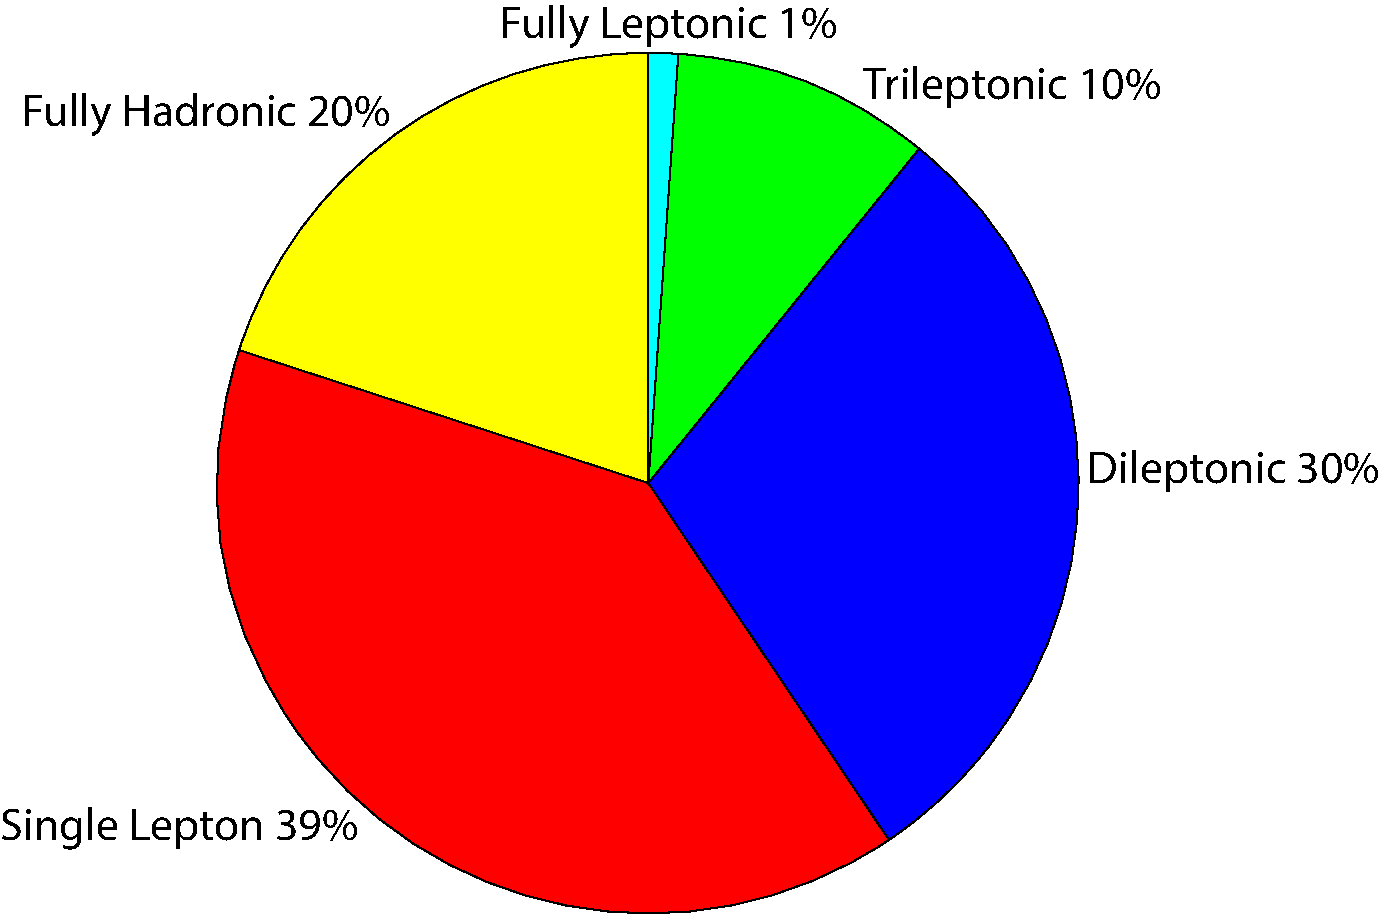
\includegraphics[width=0.5\textwidth]{images/Analysis/FourTopBR.pdf}
    \caption{The possible decay channels for \tttt production}
    \label{fig:ttttDecay}
\end{figure}




\section{Calibrations of the simulation}
\label{sec:Calibrations}
Many of the parameters which go into making simulation for each particle physics process are not precisely known therefore they are tuned to produce the simulation which best matches the data observed. This simulation will still have discrepancies from data which can be measured and accounted for by producing \emph{scale factors} which adjust the weight of each event in the simulation such that the overall distributions more closely match data. 


\subsection{Pileup reweighting}
\label{sec:pile-up}
The distribution of the number of primary vertices varies between data and simulation. This can be taken into account by looking at the number of events for each number of primary vertices in data and simulation and applying the scale factor, $SF_{PU}\left( i \right)$ to simulation, where \emph{i} is the number of vertices.

\begin{equation}
SF_{PU}\left( i \right) = \frac{N_{events}^{Data}}{  N_{events}^{simu}} 
\label{eqn:PUSF}
\end{equation}

\subsection{b tag modelling}

There are significant differences between b tag efficiencies measured by CMS in data and the efficiencies as measured in simulation. To account for this, a weight must be applied to the selected MC events in order to predict the correct event yield in data. The full method can be found in this reference~\cite{CMS-PAS-BTV-13-001}.

\subsection{Heavy flavour jet modelling}

There is a discrepancy between data and simulation in the tails of the \fxnote*{show unweighted}{distribution} of the number of b-tagged jets (\nbtags) which suggests that the amount of heavy flavour jets in \ttbar events is incorrectly simulated. The ratio of \heavyflavour was measured by CMS to be $2.2 \pm 0.3 \left( \textrm{stat.} \right) \pm 0.5 \left(\textrm{sys.} \right)\% $ ~\cite{CMS:2014yxa} at $\sqrt{s} =$ 8TeV. To incorporate this ratio into the analysis, the MC truth information of the \ttbar$+$jets MC sample is used to split the sample into \ttbb, \ttcc and \ttll, where l denotes light quarks and gluons (\cPqu, \cPqd, \cPqs, \cPg) . Weights are applied to each sub-sample to match the measured ratio whilst preserving the total number of \ttbar events. After this procedure is applied, the agreement between data and simulation in the \nbtags distribution is improved as can be seen in Fig~\ref{fig:datasimnbtags}.

\subsection{Lepton modelling}
Due to a difference between data and simulation in the efficiency of lepton identification and isolation, a weight is applied to events which is dependent on the selected leptons $\eta$, $\pt$ and lepton flavour.

\section{Multi-jet background estimation}
\label{sec:QCDbackground}
The presence of multi-jet events within the signal region defined by the baseline selection is investigated in this section. It is rare for multi-jet events to have a highly energetic undetectable particle. Therefore, the $\MET$ distributions for multi-jet events typically peak at \fxnote*{more specific?}{low values}. It can be seen from the MET distributions in Fig.~\ref{fig:datasimMET} that the data agrees well with the simulation at low values which suggests there are very few multi-jet events which pass the tight requirements in the baseline selection. Due to this small number of events, it is not possible to use multi-jet MC to estimate this background. In this case, a data-driven method known as the \fxnote*{ref?}{ABCD method} may be used. This method proceeds by selecting two uncorrelated variables from the object or baseline selection and defining three control regions (A,B,C) and one signal region (D) in the 2-dimensional phase space of these variables. The event variable \MET and the lepton variable RelIso were selected as they are \fxnote*{uncorrelated proof??}{uncorrelated} and the defined regions are shown below. Trigger requirements place an upper bound on the RelIso which restricts the region choice.\\











\section{Multi-variate analysis techniques}
\subsection{Boosted Decision Trees}
\label{sec:BDT}


\subsection{Reconstruction of hadronic top quarks}

\subsection{Event-level BDT}

\section{Limit setting}

\subsection{Categorisation}
\label{sec:Categorisation}






\chapter{The search for standard model~\tttt production in \runone at $\sqrt{s} =$ 8TeV }
\label{c:Run1}

\section{Introduction}
In this chapter, an analysis of the full 2012 CMS dataset at $\sqrt{s} =$ 8TeV with 19.7 \fbinv of data is presented where the Standard Model production of four top quarks (\tttt) is sought. Standard model \tttt production has a cross section of $\sigmattttSM \approx 1.3$ fb at NLO with NNLO corrections~\cite{Barger201070,Bevilacqua2012}. 

% this equates to approximately 26 events in the 2012 dataset in all decay channels. However, in this analysis, only final states where one of the top quarks decays leptonically into an electron or muon are considered. These are referred to as the single lepton channels and they are the most prevalent decay mode as can be seen in ~\fxnote*{add fig}{figX}. One of the main challenges of this analysis is to distinguish this extremely rare signal process with the overwhelmingly large background process of top-pair production (\ttbar) which is five orders of magnitude greater than the \tttt signal process, the latest measurement putting it at $241.5 \pm 8.5$ \pbinv ~\cite{CMS-PAS-TOP-14-016}. 


%This analysis proceeds as follows; Section~\ref{sec:sigback} discuss the \tttt signal processes and the relevant background and Section~\ref{sec:datasimulation} describes the datasets and simulations of the signal and backrgound used. Section~\ref{sec:baseline} details the initial requirements imposed on the signal region while Section~\ref{sec:Calibrations} describes the calibrations made to the correct the simulation. The multi-jet background estimation is described in Section~\ref{sec:QCDbackground} and the multi-variate techniques used to increase the discrimination power between signal and background are contained in~\ref{sec:discriminating}. Discussion of the systematic uncertainties and extraction of the limit on the \tttt cross section are in Sections~\ref{sec:uncertainties} and~\ref{sec:limit}. Validation of the analysis can be found in Section~\ref{sec:signalinjection}. Finally, a summary and discussion of the ATLAS \tttt cross section limit can be found in Sections~\ref{sec:summary} and~\ref{sec:ATLASresult}.
Sections~\ref{sec:QCDbackground},~\ref{sec:njetcatlimit} and~\ref{sec:signalinjection} are the authors personal contribution to the analysis.

%An initial baseline selection of requirements on the number of leptons, jets, b-tagged jets, transverse hadronic energy (\HT) and transverse missing energy (\MET) reduces the \ttbar background to three orders of magnitude greater than the \tttt signal. As \ttbar remains a very large background, multi-variate techniques are employed to reconstruct top quarks and then ultimately to find a discriminator value to distinguish between signal and background.
%In the absence of an excess of events over background, the \CLS method is used to obtain an observed limit on the cross section of \tttt production of 32 fb at 95\% confidence level compared to 32$\pm17$ fb expected.



\section{Data and Simulation}
\label{sec:datasimulation}
This analysis uses data from proton-proton collision at the CMS experiment in 2012 at $\sqrt{s}=8$~TeV.
For the muon (electron) channel, the data were collected using a trigger based on the presence of at least one muon (electron) candidate with $\pt > $ 24 (27) GeV and corresponds to an integrated luminosity of 19.7 \fbinv .
% The full 2012 SingleElectron dataset is used for the electron channel, which requires an electron candidate with $\pt > $ 27 GeV and corresponds to an integrated luminosity of 19.7 \fbinv.
The signal SM \tttt Monte Carlo (MC) samples and the background MC samples are given in table~\ref{tab:datasets_sim_8tev}, along with the MC generator used to produce these samples, the order at which they were produced and the number of events produced. MC samples were produced for the scale and matching systematics, these can be found in table~\ref{tab:datasets_sys_8tev}. In this analysis the scale uncertainty includes the ME scale and PS scale.


\begin{table}[ht!]
% \tiny
\centering
\begin{tabular}{| l | l | l | p{2cm} |}
 \hline 
 Dataset & Events & Generator & Order \\
\hline
TTTT & 100K & Madgraph  $+$ Tauola& O \\
\hline
TTJets\_SemiLeptMGDecays &25M & Madgraph $+$ Tauola & O \\
\hline
TTJets\_HadronicMGDecays &31M & Madgraph  $+$ Tauola& O \\
\hline
TTJets\_FullLeptMGDecays\ & 12M & Madgraph  $+$ Tauola& O \\
\hline
W4JetsToLNu & 13M & Madgraph & O \\
\hline
Tbar\_tW-channel & 500K & Powheg $+$ Tauola & O\\
\hline
T\_tW-channel & 500K & Powheg $+$ Tauola & O \\
\hline
T\_t-channel & 3.8M & Powheg $+$ Tauola & O \\
\hline
Tbar\_s-channel & 260K & Powheg $+$ Tauola & O \\
\hline
T\_s-channel & 139K & Powheg $+$ Tauola & O \\
\hline
Tbar\_t-channel & 2M  & Powheg $+$ Tauola & O \\
\hline
DY4JetsToLL & 6.2M & Madgraph & O  \\
\hline
DYJetsToLL & 6.7M & Madgraph & O \\
\hline
TTZJets  & 200K & Madgraph & O \\
\hline
TTWJets\ & 200K & Madgraph & O \\
\hline
TTH\_HToBB & 1M & Pythia6 $+$ Tauola & O \\
\hline
ZZ & 10M & Pythia6 $+$ Tauola & O \\
\hline
WZ &10M & Pythia6 $+$ Tauola & O \\
\hline
WW &10M & Pythia6 $+$ Tauola & O \\
\hline
\end{tabular}
 \caption{Dataset name, total number of events, MC generator and order of the simulated samples.}
  \label{tab:datasets_sim_8tev}
  \end{table}


\begin{table}[ht!]
% \tiny
\centering
\begin{tabular}{| l | l | l | p{2cm} |}
 \hline 
 Dataset & Events & Generator & Order \\
\hline
TTJets\_scaledown & 5M  & Madgraph $+$ Tauola & O \\
\hline
TTJets\_scaleup & 5M  & Madgraph $+$ Tauola & O \\
\hline
TTJets\_matchingdown & 5M & Madgraph $+$ Tauola & O  \\
\hline
TTJets\_matchingup & 5M & Madgraph $+$ Tauola & O \\
\hline
\end{tabular}
 \caption{Dataset name, total number of events, MC generator and order of the simulated systematic samples.}
  \label{tab:datasets_sys_8tev}
\end{table}

\section{Baseline Event Selection}
\label{sec:baseline}
To select \tttt events and suppress background events, a set of criteria is applied to the reconstructed objects in events which are triggered by the single muon or single electron triggers.
For the muon channel these are:
\begin{itemize}
\setlength\itemsep{0em}
\item Exactly one tight muon
\item Exactly zero additional loose muons
\item Exactly zero loose electrons
\item At least 6 jets with $\pt >$ 30 \GeV
\item At least 2 CSVM tagged b-jets
\item $\HT > $ 400 \GeV 
\item $\MET > $ 30 \GeV 
\end{itemize}
For the electron channel these are:
\begin{itemize}
\itemsep0em 
\item Exactly one tight electron
\item Exactly zero additional loose electrons
\item Exactly zero loose muons
\item At least 6 jets with $\pt >$ 30 \GeV
\item At least 2 CSVM tagged b-jets
\item $\HT > $ 400 \GeV 
\item $\MET > $ 30 \GeV 
\end{itemize}

\section{Corrections to the simulation}
\label{sec:Calibrations8}
All corrections are described in section~\ref{sec:Calibrations}.
The events for all background and signal samples which pass the baseline event selection are given a weight which is the product of the weight for the pile up corrections, a weight to correct the b-tag modelling from the method in ~\ref{subsec:method1btag} and a weight for lepton modelling corrections. The heavy flavour jet modelling from section~\ref{ttbbmod} is applied to the \ttbar background.



% \subsection{b tag modelling}

% There are significant differences between b tag efficiencies measured by CMS in data and the efficiencies as measured in simulation. To account for this, a weight must be applied applied to the selected MC events in order to predict the correct event yield in data. The full method can be found in this reference~\cite{CMS-PAS-BTV-13-001}.

% \subsection{Heavy flavour jet modelling}

% There is a discrepancy between data and simulation in the tails of the \fxnote*{show unweighted}{distribution} of the number of b-tagged jets (\nbtags) which suggests that the amount of heavy flavour jets in \ttbar events is incorrectly simulated. The ratio of \heavyflavour was measured by CMS to be $2.2 \pm 0.3 \left( \textrm{stat.} \right) \pm 0.5 \left(\textrm{sys.} \right)\% $ ~\cite{CMS:2014yxa} at $\sqrt{s} =$ 8TeV. To incorporate this ratio into the analysis, the MC truth information of the \ttbar$+$jets MC sample is used to split the sample into \ttbb, \ttcc and \ttll, where l denotes light quarks and gluons (\cPqu, \cPqd, \cPqs, \cPg) . Weights are applied to each sub-sample to match the measured ratio whilst preserving the total number of \ttbar events. After this procedure is applied, the agreement between data and simulation in the \nbtags distribution is improved as can be seen in Fig~\ref{fig:datasimnbtags}.

% \subsection{Lepton modelling}
% Due to a difference between data and simulation in the efficiency of lepton identification and isolation, a weight is applied to events which is dependent on the selected leptons $\eta$, $\pt$ and lepton flavour.
\section{Weighted event counts through baseline event selection \label{cutflow}}

The event counts weighted by the various corrections in section~\ref{sec:Calibrations8} are given for the muon (electron) channel in table~\ref{tab:museltable8} (table~\ref{tab:eseltable8}). It is quite evident that the main background is \ttbar production, with smaller contributions coming from W$+$jets, Z$+$jets and single top (ST) as well as almost negligible contributions from the diboson and TT+X background (X $=$ H, Z, W).
\fxnote {discuss grouping of backgrounds}




\begin{table}
\tiny
\caption{Cut flow for the $\mu$ + jets channel ($19695.0~pb^{-1}$ of int. lumi.)}
\label{tab:museltable8}
\centering
\begin{tabular}{|c|c|c|c|c|c|c|c|c|c|c|c|c|}
\hline
&$Data$ &$\tttt$  &$ttH$  &$Wjets$ &$Zjets$ &$ST$ &$WW$ &$WZ$ &$ZZ$ &$TTZ$  &$TTW$  &$\ttbar$ \\
\hline
Trigger&  120508.0  &4.5  &171.8  &16094  &3916.3 &3256.2 &272.0  &161.1  &71.5 &219.3  &277.5  &84476  \\

1 iso. $\mu$& 95723.0 &3.5  &141.6  &13655  &2635.1 &2750.2 &232.7  &125.0  &47.6 &168.5  &229.3  &70030  \\

Loose $\mu$ veto& 93385.0 &3.2  &138.9  &13654  &1835.3 &2739.2 &232.3  &114.7  &34.0 &153.5  &222.9  &69503  \\

Loose e veto& 91546.0 &2.5  &132.6  &13593  &1812.0 &2691.6 &228.9  &113.0  &33.3 &143.6  &206.0  &68040  \\

$>$= 6 Jets&  24791.0 &2.3  &59.1 &2428.4 &350.7  &591.9  &41.5 &20.0 &5.1  &71.8 &94.1 &21197  \\

$>$= 2 b-tags&  9260.0  &1.7  &46.0 &68.8 &15.2 &215.5  &3.1  &1.4  &0.6  &35.0 &39.5 &9138.8 \\

HT $>$=  400 GeV& 6342.0  &1.6  &37.7 &49.3 &10.4 &156.9  &2.6  &1.0  &0.4  &29.6 &32.8 &6542.2 \\

\MET $>$=  30 GeV&      5215.0  &1.5    &31.7   &41.5   &7.1    &132.2  &2.2    &0.9    &0.1    &24.4   &28.3   &5415.1 \\
\hline
\end{tabular}
\end{table}



\begin{table}
\tiny
\caption{Cut flow for the $e$ + jets channel ($19721.7~pb^{-1}$ of int. lumi.)}
\label{tab:eseltable8}
\centering
\begin{tabular}{|c|c|c|c|c|c|c|c|c|c|c|c|c|c|}
\hline
&$Data$ &$\tttt$  &$ttH$  &$Wjets$ &$Zjets$ &$ST$  &$WW$ &$WZ$ &$ZZ$ &$TTZ$  &$TTW$  &$\ttbar_{other}$ &$\ttbar_{semi-lep}$  \\
\hline
Trigger and PV& $1128500$ &$8.6$  &$307.8$  &$28831$  &$25118.7$  &$6494.4$ &$683.8$  &$464.1$  &$228.3$  &$440.4$  &$545.5$  &$14569$  &$157087$ \\

1 iso. e& $103856$  &$3.2$  &$117.6$  &$9631.6$ &$7183.4$ &$2212.4$ &$217.6$  &$136.8$  &$60.9$ &$156.4$  &$207.4$  &$5050$ &$59293$  \\

Loose e veto& $100861$  &$3.0$  &$115.9$  &$9611.2$ &$5354.2$ &$2199.2$ &$216.4$  &$121.7$  &$43.7$ &$144.7$  &$201.9$  &$4611$ &$59201$  \\

Loose mu veto&  $99402$ &$2.3$  &$110.9$  &$9605.0$ &$5340.7$ &$2172.0$ &$215.2$  &$120.8$  &$43.3$ &$134.4$  &$186.3$  &$3456$ &$59128$  \\

$>$= 6 Jets&  $26508$ &$2.1$  &$55.2$ &$1660.3$ &$1108.3$ &$490.7$  &$32.0$ &$20.6$ &$7.2$  &$67.6$ &$84.7$ &$977.8$  &$18799$  \\

$>$= 2 b-tags&  $8945$  &$1.5$  &$43.2$ &$45.4$ &$19.8$ &$179.3$  &$1.3$  &$2.0$  &$0.8$  &$31.5$ &$35.6$ &$421.1$  &$7941$ \\

HT $>$= 400 GeV&  $6278$  &$1.5$  &$35.6$ &$33.2$ &$13.9$ &$134.2$  &$1.0$  &$1.3$  &$0.5$  &$26.1$ &$29.1$ &$321.4$  &$5739.7$ \\

\MET $>$ 30 GeV & $5066$  &$1.3$  &$30.0$ &$25.4$ &$7.0$  &$114.2$  &$0.8$  &$1.1$  &$0.2$  &$21.5$ &$24.5$ &$297.0$  &$4676.9$ \\
\hline
\end{tabular}
\end{table}




\section{Data-simulation agreement}

% After the baseline event selection, events are weighted using the prescription for pile-up as described in Section~\ref{sec:pile-up}. The weights are applied for b-tagging, the heavy flavour jet modelling and the lepton modelling as described in Section~\ref{sec:run1:baseline}. 

The distributions which show the data-simulation agreement for \njets, \nbtags, \HT and \MET after these weights are applied are shown in Figs~\ref{fig:datasimnjets},~\ref{fig:datasimnbtags},~\ref{fig:datasimHT},~\ref{fig:datasimMET}. As the scale uncertainty is the largest uncertainty on the background, it is shown as a hatched error band on the distributions. It can be seen that there is good agreement between data and simulation in these distributions and that the signal (overlaid and multiplied by 100 for visibility) has a different shape in these variables in the background processes particularly in the \njets, \nbtags, \HT which make them viable candidates to be used in the event-level BDT.

\fxnote{Get version of plots from papers with bigger titles}

\begin{figure}[ht!]
\centering
    \includegraphics[width=0.49\textwidth]{images/Run1/NbOfSelectedJets_mu.pdf}
     \includegraphics[width=0.49\textwidth]{images/Run1/NbOfSelectedJets_e.pdf}       
    \caption{Data-simulation comparison for \njets for $\mu$ + jets (right) and e + jets (left).}
    \label{fig:datasimnjets}
\end{figure}

\begin{figure}[ht!]
\centering
    \includegraphics[width=0.49\textwidth]{images/Run1/NbOfSelectedBJets_mu.pdf}
     \includegraphics[width=0.49\textwidth]{images/Run1/NbOfSelectedBJets_e.pdf}        
    \caption{Data-simulation comparison for \nbtags for $\mu$ + jets (right) and e + jets (left).}
    \label{fig:datasimnbtags}
\end{figure}

\begin{figure}[ht!]
\centering
    \includegraphics[width=0.49\textwidth]{images/Run1/HT_SelectedJets_StackLogY_Mu.pdf}
     \includegraphics[width=0.49\textwidth]{images/Run1/HT_SelectedJets_StackLogY_e.pdf}          
    \caption{Data-simulation comparison for \HT for $\mu$ + jets (right) and e + jets (left). }
    \label{fig:datasimHT}
\end{figure}

\begin{figure}[ht!]
\centering
    \includegraphics[width=0.49\textwidth]{images/Run1/MET_StackLogY_Mu.pdf}
     \includegraphics[width=0.49\textwidth]{images/Run1/MET_StackLogY_e.pdf}          
    \caption{Data-simulation comparison for \MET for $\mu$ + jets (right) and e + jets (left). }
    \label{fig:datasimMET}
\end{figure}



\section{Multi-jet background estimation}
\label{sec:QCDbackground}
The presence of multi-jet events within the signal region defined by the baseline selection is investigated in this section. 
%It is rare for multi-jet events to have a highly energetic undetectable particle. Therefore, the $\MET$ distributions for multi-jet events typically peak at \fxnote*{more specific?}{low values}. 
It can be seen from the MET distributions in Fig.~\ref{fig:datasimMET} that the data agrees well with the simulation at low values which suggests there are very few multi-jet events which pass the tight requirements in the baseline selection. 
%Due to this small number of events, it is not possible to use multi-jet MC to estimate this background. In this case, a data-driven method known as the \fxnote*{ref?}{ABCD method} may be used. This method proceeds by selecting two uncorrelated variables from the object or baseline selection and defining three control regions (A,B,C) and one signal region (D) in the 2-dimensional phase space of these variables. The event variable \MET and the lepton variable RelIso were selected as they are \fxnote*{uncorrelated proof??}{uncorrelated} and 
The defined regions in the uncorrelated variables of \MET and $RelIso$ are shown below. The upper bound in $RelIso$ is restricted by the minimum $RelIso$ values required by the HLT in the single muon and single electron streams.\\

For the muon channel these are:
\begin{itemize}
\setlength\itemsep{0em}
\item A : 30 $<\MET<$ 500, 0.1 $<$ RelIso $<$ 0.15
\item B : 0 $<\MET<$ 30, 0.1 $<$ RelIso $<$ 0.15
\item C : 0 $<\MET<$ 30, 0 $<$ RelIso $<$ 0.1
\item D : 30 $<\MET<$ 500, 0 $<$ RelIso $<$ 0.1
\end{itemize}
For the \eplusjets:
\begin{itemize}
\itemsep0em
\item A : 30 $<\MET<$ 500, 0.12 $<$ RelIso $<$ 0.2
\item B : 0 $<\MET<$ 30, 0.12 $<$ RelIso $<$ 0.2
\item C : 0 $<\MET<$ 30, 0 $<$ RelIso $<$ 0.12
\item D : 30 $<\MET<$ 500, 0 $<$ RelIso $<$ 0.12
\end{itemize}

%It is assumed that the multi-jet background can be estimated from the data minus the background expectation from all of the other MC samples considered in Section~\ref{sec:datasimulation}. 
The results of the background subtraction from data and the defined ABCD regions are shown in Fig.~\ref{fig:QCDplots}.
The number of multi-jet events, N$_{\textrm{multi-jet}}$, in each of the control regions are used to predict the number of multi-jet events in region D using Eq.~\ref{N-multi-jet}, the results of which are shown in Table~\ref{tab:multijet}.

\begin{figure}[!ht]
    \includegraphics[width=0.49\textwidth]{images/Run1/Data_Minus_MC_Mu-1.pdf}
    \includegraphics[width=0.49\textwidth]{images/Run1/Data_Minus_MC_El.pdf}
    \caption{Data minus MC background for MET vs lepton iso for $\mu$ + jets (right) and e + jets (left).}
    \label{fig:QCDplots}
\end{figure}


\begin{equation}
\frac{\textrm{N}^{\textrm{B}}_{\textrm{multi-jet}}}{\textrm{N}^{\textrm{A}}_{\textrm{multi-jet}}} = \frac{\textrm{N}^{\textrm{C}}_{\textrm{multi-jet}}}{\textrm{N}^{\textrm{D}}_{\textrm{multi-jet}}}
\label{N-multi-jet}
\end{equation}

\begin{table}[ht!]
\caption{Multi-jet estimation}
\centering
\begin{tabular}{|c |c |c |c |c |}
 \hline 
 Channel & N$^{\textrm{A}}_{\textrm{multi-jet}}$  & N$^{\textrm{B}}_{\textrm{multi-jet}}$ & N$^{\textrm{C}}_{\textrm{multi-jet}}$ & Prediction for N$^{\textrm{D}}_{\textrm{multi-jet}}$  \\
  \hline
$\mu$ + jets & 19.1 & 16.1 & -16.8 & -20  \\
 \hline
$e$ + jets & 36.8  & 50.8 & 62.7 &45.5  \\
\hline
\end{tabular}
\label{tab:multijet}
\end{table}

As the the number of \ttbar events in simulation has fluctuated to be greater than the data in region C in the muon channel, the prediction for the signal region D is negative. As this prediction is unphysical, the number of events is estimated to be zero in the muon channel. In the electron, 45.5 multi-jet events are predicted which is considered negligible at $<1\%$ of the massive \ttbar background. Hence, the multi-jet background is not considered further.
\fxnote{scale up scale down...200\% uncertainty?}

\section{Discriminating between signal and background}
\label{sec:discriminating}
The dominant background process after the baseline selection is \ttbar production. It is three orders of magnitude greater than the \tttt signal process in the signal region. This motivates the search for variables which can discriminate between these two processes. There are three main features which can be used to discriminate; the number of top quarks which can be reconstructed in the event, the number of b-jets found in each event, and event activity such as \HT.

\subsection{Top quark content}
\label{sec:topContent}
In the single lepton channel for \tttt production, there are three top quarks where the W boson decays hadronically, these will be referred to as hadronic top quarks. For the main background of \ttbar there is only one hadronic top quark. Additional jets in \ttbar come from \fxnote*{assume previously defined}{ISR or FSR} in order to satisfy the requirements of the baseline selection. Therefore, it should only be possible to reconstruct more than one top quark from three jets originating from it's hadronic decay in \tttt but not in \ttbar. However, the \antikt algorithm can only distinguish separate jets if they have \DR$>0.5$ between them, hence it may not always be possible to reconstruct all hadronic top quarks. To ascertain whether this might be a powerful technique for separating \tttt and \ttbar or not, 1000 \tttt and 1000 \ttbar events were analysed where there was one muon with \PT $>$ 26 GeV and exactly 6 jets with \PT $>$ 30 and $\lvert \eta \rvert<$ 2.5. Hadronic top quarks are considered reconstructible at parton level if they decayed into jets with \DR  $>$  0.5. The number of reconstructible hadronic top quarks for \tttt and \ttbar are shown in Fig.~\ref{fig:ReconHadTops}.

\begin{figure}[!ht]
    \includegraphics[width=0.6\textwidth]{images/Run1/ReconstructibleTops.pdf}
    \caption{The number of reconstructible hadronic top quarks in \tttt and \ttbar}
    \label{fig:ReconHadTops}
\end{figure}

For \tttt production at parton level it is possible to reconstruct more than one hadronic top quark $\approx$ 63 $\%$ of the time compared to a negligible number of times in \ttbar, as is evident in the Fig.~\ref{fig:ReconHadTops}. Hence, using the number of hadronic tops can be assumed to be a powerful variable worth investigating. One obstacle to this is the large number of ways in which the jets can be combined in events with \njets $\geq 6$.\fxnote{more on combinatorics? -> but James' work} This motivates the use of multi-variate analysis to distinguish between good tri-jet combinations and bad tri-jet combinations, where a tri-jet refers to any given combination of three jets. Figure~\ref{fig:TopBDTinput} shows the minimal number of discriminating variables which are used including:\\
\textbf{Tri-jet invariant mass} - Good tri-jet combinations should have an invariant mass distribution which peaks around the top mass.\\
\textbf{Di-jet invariant mass} - The di-jet combination is formed from the two jets with the smallest \DR separation. The invariant mass distribution should peak around the W mass.\\
\textbf{\ptrat} - This is the ratio of the vectorial \pt to the scalar sum of the \pt of the jets in the tri-jet combination.\\
\textbf{\DPTW} - This is the \Dphi separation between the tri-jet and di-jet system.\\
\textbf{\DPTb} - This is the \Dphi separation between the tri-jet and remaining jet not included in the di-jet system.\\
\textbf{\CSVj} - For the jet not used in the di-jet system, the CSV b-tagging discriminator value is used.\\

\begin{figure}[ht!]
\centering
    \includegraphics[width=0.49\textwidth]{images/Run1/TriJetMass.pdf}
     \includegraphics[width=0.49\textwidth]{images/Run1/HadWMass.pdf}
    \includegraphics[width=0.49\textwidth]{images/Run1/ThSumPTVecPT.pdf}
     \includegraphics[width=0.49\textwidth]{images/Run1/AnThWh.pdf}
    \includegraphics[width=0.49\textwidth]{images/Run1/AnThBh.pdf}
     \includegraphics[width=0.49\textwidth]{images/Run1/BTag.pdf}          
    \caption{Input variables into top quark reconstruction BDT.}
    \label{fig:TopBDTinput}
\end{figure}

The multi-variate analysis tool chosen to calculate a variable to discriminate between good and bad tri-jet combinations is a BDT. The BDT is described in more detail in Section~\ref{sec:BDT}. The distribution of the discriminator variable which is output from the BDT is shown in Fig.~\ref{fig:TopBDToutput} where the features in the shape are caused by the large discriminating power of the tri-jet and di-jet invariant mass.
\begin{figure}[!ht]
\centering
    \includegraphics[width=0.6\textwidth]{images/Run1/BDT_Disc.pdf}
    \caption{Output discriminator variable from top quark reconstruction BDT}
    \label{fig:TopBDToutput}
\end{figure}

\subsubsection*{Multitopness}
Multitopness is defined to be the BDT discriminator value of the second highest ranking tri-jet after the first highest-ranking tri-jet has been removed from the collection and the remaining jets have been passed through the BDT again. The multitopness value should have values close to 1 for events where there is a second reconstructible top and a value close to -1 where there is only one reconstructible top which has been removed from the collection and the remaining jets are from ISR or FSR. The distributions of the multitopness variable are shown in Fig.~\ref{fig:Multitopness} for the muon and electron channel. It can be seen that the data and simulation agree well and there is some difference between the shape of the signal and background distributions. The interesting features in the distributions shape come from the the BDT. The two strongest variables, the tri-jet invariant mass and the di-jet invariant mass, split the dataset sharply into two and then four main sections.

\begin{figure}[!ht]
    \includegraphics[width=0.49\textwidth]{images/Run1/MultiTopness_Mu.pdf}
    \includegraphics[width=0.49\textwidth]{images/Run1/MultiTopness_e.pdf}
    \caption{Multitopness variable in data and simulation for $\mu$ + jets (right) and e + jets (left).}
    \label{fig:Multitopness}
\end{figure}

\subsubsection*{Reduced Event Variables}
New event variables are constructed from removing the highest ranking tri-jet from the jets collection to created a reduced event. These reduced event variables exploit the fact the \ttbar events should only have softer jets remaining from ISR and FSR, whereas \tttt events should have ore energetic jets from the two additional hadronic top quarks.

\textbf{\HTX} - This is the \HT of the reduced event.\\
\textbf{\sumjetmassX} - Invariant mass of all jets contained in the reduced event.

Plots for these reduced event variables can be seen in Figs~\ref{fig:HTX},~\ref{fig:sumjetmassX}.

\begin{figure}[!ht]
    \includegraphics[width=0.49\textwidth]{images/Run1/HTX_StackLogY_Mu.pdf}
    \includegraphics[width=0.49\textwidth]{images/Run1/HTX_StackLogY_e.pdf}
    \caption{\HTX for $\mu$ + jets (right) and e + jets (left).}
    \label{fig:HTX}
\end{figure}

\begin{figure}[!ht]
    \includegraphics[width=0.49\textwidth]{images/Run1/SumJetMassX_StackLogY_Mu.pdf}
    \includegraphics[width=0.49\textwidth]{images/Run1/SumJetMassX_StackLogY_e.pdf}
    \caption{\sumjetmassX for $\mu$ + jets (right) and e + jets (left).}
    \label{fig:sumjetmassX}
\end{figure}

\subsection{b-jet content}
\label{sec:bottomContent}
Top quarks decay almost exclusively into bottom quarks by \cPqt $\rightarrow$ \cPqb \Wplus or \cPaqt $\rightarrow$ \cPaqb \Wminus. Therefore, it should be possible to use the number of bottom quarks in the event to distinguish between \tttt events, which should have four bottom quarks in comparison to \ttbar + jets events which typically have two bottom quarks. However this variable does not help to distinguish between \tttt and \ttbb as \ttbb will also have four bottom quarks in the final state. Also \ttbar + jets may have additional bottom quarks arising from the ISR or FSR. Fig~\ref{fig:datasimnbtags} shows the distribution of \nbtags.

\subsection{Event activity}
\label{sec:eventActivity}
Many variables can be derived by utilising the fact that \tttt events can have up to 10 hard jets whereas \ttbar events should only have up to 4 hard jets. This difference in hadronic activity is exploited by forming the following variables:\\
\textbf{\njets} - The number of jets is an obvious variable for distinguishing between \tttt and \ttbar. It can be seen in Fig.~\ref{fig:datasimnjets}. \\
\textbf{\HTb} - The scalar sum of the \pt of the b-tagged jets in the event. Bottom quarks which come from top quark decays tend to have higher \pt than bottom quarks which come from gluon splitting and other processes. As \tttt events should contain four b-quarks which come from top decays and \ttbar events contain two b-quarks from top decays, this variable should be larger for \tttt events, as can be seen in Fig.~\ref{fig:HTb}.\\
\textbf{Centrality} - This is defined as the ratio of the \HT in the event to the H in the event, where H is the scalar sum of the total momentum (P) in the event.\\
\textbf{\HTrat} - This is defined as the ratio of the \HT of the four leading jets to the \HT of the other jets in the event. For \ttbar, which should have only four hard jets, this ratio should be larger than \tttt which should have a value closer to one as the four hardest jets are balanced be additional hard jets in the event. \\
\textbf{5th jet \pt} - After the four leading hard jets in \ttbar, the 5th jet should have, on average, a lower momentum in \ttbar events than in \tttt events. This can be seen in Fig.~\ref{fig:5thjetpt}.\\
\textbf{6th jet \pt} - Again, the \pt of the 6th jet in \ttbar events should be, on average, lower than in \tttt where the 6th jet is still coming from a hard process. This can be seen in Fig.~\ref{fig:6thjetpt}.\\

\begin{figure}[!ht]
    \includegraphics[width=0.49\textwidth]{images/Run1/HTb_SelectedJets_StackLogY_Mu.pdf}
    \includegraphics[width=0.49\textwidth]{images/Run1/HTb_SelectedJets_StackLogY_e.pdf}
    \caption{\HTb for $\mu$ + jets (right) and e + jets (left).}
    \label{fig:HTb}
\end{figure}

\begin{figure}[!ht]
    \includegraphics[width=0.49\textwidth]{images/Run1/HTH_StackLogY_Mu.pdf}
    \includegraphics[width=0.49\textwidth]{images/Run1/HTH_StackLogY_e.pdf}
    \caption{Centrality for $\mu$ + jets (right) and e + jets (left).}
    \label{fig:HTrat}
\end{figure}

\begin{figure}[!ht]
    \includegraphics[width=0.49\textwidth]{images/Run1/HTRat_StackLogY_Mu.pdf}
    \includegraphics[width=0.49\textwidth]{images/Run1/HTRat_StackLogY_e.pdf}
    \caption{\HTrat for $\mu$ + jets (right) and e + jets (left).}
    \label{fig:HTrat}
\end{figure}

\begin{figure}[!ht]
    \includegraphics[width=0.49\textwidth]{images/Run1/5thJetPt_StackLogY_Mu.pdf}
    \includegraphics[width=0.49\textwidth]{images/Run1/5thJetPt_StackLogY_e.pdf}
    \caption{5th jet \pt for $\mu$ + jets (right) and e + jets (left).}
    \label{fig:5thjetpt}
\end{figure}

\begin{figure}[!ht]
    \includegraphics[width=0.49\textwidth]{images/Run1/6thJetPt_StackLogY_Mu.pdf}
    \includegraphics[width=0.49\textwidth]{images/Run1/6thJetPt_StackLogY_e.pdf}
    \caption{6th jet \pt for $\mu$ + jets (right) and e + jets (left).}
    \label{fig:6thjetpt}
\end{figure}

\subsection{Event-level BDT}
All of the variables described in Sections~\ref{sec:topContent},~\ref{sec:bottomContent} \&~\ref{sec:eventActivity} are used in a BDT, known as the event-level BDT. It is necessary to use a sample of events which were not used to train the kinematic reconstruction of top quarks to train the event-level BDT so that an orthogonal training sample can be provided. An additional set of events are used to test the performance of the BDT. The output distribution of the BDT discriminator can be seen in Fig.~\ref{fig:BDT}.

\begin{figure}[!ht]
    \includegraphics[width=0.49\textwidth]{images/Run1/MVA_Mu.pdf}
    \includegraphics[width=0.49\textwidth]{images/Run1/MVA_e.pdf}
    \caption{BDT discriminator variable in data and simulation for $\mu$ + jets (right) and e + jets (left).}
    \label{fig:BDT}
\end{figure}

\section{Systematic uncertainties}
\label{sec:uncertainties}
There are two categories of systematic uncertainties; (i) Uncertainties which affect the normalisation of the distributions which are applied to signal and background and (ii) uncertainties which affect the shape of the distributions which are applied to the dominant background, in this case \ttbar. 
\subsection{Normalisation uncertainties}
%The normalisation uncertainties will only affect the uncertainty on the expected limit rather than the limit itself when it is used in the template fit and limit setting procedure described in Section~\ref{sec:limit}.
Normalisation uncertainties include the following:
\begin{itemize}
\item \textbf{Luminosity}
The CMS Luminosity Group give a recommendation of 2.6$\%$ uncertainty on the luminosity~\cite{CMS-PAS-LUM-12-001}.
\item \textbf{Monte Carlo cross sections}
As \ttbar is the main background to \tttt, the uncertainty on its MC cross-section is expected to be dominant over the other background processes. The uncertainty on \ttbar is ${}^{+2.5\%}_{-3.4\%} \left( \textrm{renormalisation and factorisation scale} \right)$ and ${}^{+2.5\%}_{-2.6\%} \left( \textrm{PDF} \right)$~\cite{PhysRevLett.110.252004}.
\fxnote*{??}{The MC cross section uncertainties are modelled by assigning a $4\%$ uncertainty to each background process and a $10\%$ uncertainty to the signal process}
\end{itemize}

\subsection{Shape uncertainties}
 Shape uncertainties arise from the following quantities.
 \fxnote{these quantities must be previously defined}
 \begin{itemize}
\item \textbf{Factorisation and renormalisation scales}
\item \textbf{Matching threshold}
\item \textbf{JES}
\item \textbf{JER}
\item \textbf{b tagging}
\item \textbf{Pile up}
\item \textbf{\heavyflavour modelling}
 \end{itemize}
 
The analysis procedure is repeated with \ttbar samples which have the respective quantity varied by $\pm 1 \sigma$ in order the produce new BDT templates with a deviated shape However, in the case of the matching threshold, the alternative shapes are produced by varying the matching threshold up to 40 GeV and down to 20 GeV.

\section{Template fit and upper limit}
\label{sec:limit}

An upper limit was calculated on the signal strength, \signalstrength , as no excess was observed in the data. Firstly, a template fit of the BDT distributions is made using the Combine Tool~\cite{CMS-NOTE-2011-005}, where the systematic uncertainties are modelled as nuisance parameters. Shape uncertainties are constrained using gaussian terms with exponential interpolation whereas the normalisation uncertainties are constrained using lognormal terms. For the statistical uncertainties, a lightweight version of the {Beeston and Barlow method~\cite{Conway:2011in} was used. This gives one nuisance parameter for the total MC estimate and a statistical uncertainty on each bin. The background processes are grouped into the following templates for the fit: `\ttbar' for semi-leptonic \ttbar, `electroweak' for W $+$ jets and Z $+$ jets, and `\ttbar\textunderscore other' for all other \ttbar processes. Using the \CLS method~\cite{Junk1999435,0954-3899-28-10-313} with the asymptotic approximation, the best fit values of the nuisance parameters can be obtained along with the corresponding limit on \signalstrength. The cross section limit, \sigmatttt, can be derived by multiplying the \signalstrength by \sigmattttSM $\approx 1.3$.

\subsection{Splitting into \njets categories}
\label{sec:njetcatlimit}
To increase the sensitivity of the analysis, the BDT templates were split into three \njets categories (\njets $= 6$, \njets $= 7 $ \& \njets $\geq 8$) each for the muon and electron channel. The higher \njets categories benefit from better discrimination power between signal and background as \tttt events are likely to have a larger number of jets. The \njets $= 6$ category helps to constrain the main background of \ttbar. A simultaneous fit of these three \njets categories is made for the muon channel, the electron channel and a combination of the two. The limits extracted using the \CLS method are shown in Table~\ref{tab:lims}.


\begin{table}[ht!]
\centering
\begin{tabular}{| l | l | l | p{1cm} |}
 \hline 
 Channel & Exp.  &Obs. \\
   \hline
 $\mu$ + jets & $35.6\pm 18$ & 34 \\
  \hline
$e$ + jets &  $36.1\pm16$  & 36  \\
\hline
 combined & $24.6\pm13$  & 25   \\
\hline
\end{tabular}
\hspace{0.5cm}
\begin{tabular}{| l | l | l | p{1cm} |}
 \hline 
 Channel & Exp. (fb) &Obs. (fb) \\
   \hline
 $\mu$ + jets & $46.3\pm23$ & 44 \\
  \hline
$e$ + jets &  $47.0\pm20$  & 47  \\
\hline
 combined & $32.0\pm17$  & 32   \\
\hline
\end{tabular}
\caption{CLS limits on (\sigmatttt/(\sigmattttSM) (left) and \sigmatttt (right). }
\label{tab:lims}
\end{table}

In comparison, the corresponding limit in a \fxnote*{ref PAS}{preliminary result} for a simultaneous fit of the electron and muon channels in inclusive \njets categories was observed to be 63 fb with an expected limit of  $42^{+18}_{-13}$ fb. Therefore, it can be seen that splitting into \njets categories provides a significant improvement in the sensitivity of the analysis.


\section{Signal Injection Test}
\label{sec:signalinjection}
In order to validate the limit-setting method, the following closure test was performed. A range of signal strengths were injected into the data and the limit-setting procedure was repeated as in Section~\ref{sec:limit}. Figure~\ref{fig:SigInjection} shows the BDT discriminator distributions with injected signal strengths of 20fb, 40fb and 60fb. With the increasing signal strength, there is an increase in the bins with a higher BDT discriminator values as would be expected for signal events.
\begin{figure}[ht!]
\centering
    \includegraphics[width=0.49\textwidth]{images/Run1/SignalInjection_Mu_6j.pdf}
     \includegraphics[width=0.49\textwidth]{images/Run1/SignalInjection_El_6j.pdf}
    \includegraphics[width=0.49\textwidth]{images/Run1/SignalInjection_Mu_7j.pdf}
     \includegraphics[width=0.49\textwidth]{images/Run1/SignalInjection_El_7j.pdf}
    \includegraphics[width=0.49\textwidth]{images/Run1/SignalInjection_Mu_8j.pdf}
     \includegraphics[width=0.49\textwidth]{images/Run1/SignalInjection_El_8j.pdf}          
    \caption{The BDT discriminator distributions of data and the mixtures of data and injected signal are compared for $\mu$ + jets channel $\left( \textrm{left} \right)$ and e + jets channel $\left( \textrm{right} \right)$. }
    \label{fig:SigInjection}
\end{figure}
As can be seen in Fig.~\ref{fig:SigInjectionBrazil}, the fitted value for the signal strength and observed limit increase with increasing injected singal strength as expected. However, there appears to be some bias in the analysis towards selecting background as opposed to signal as can be seen from the gradient of the line, which is $<$1.
\begin{figure}[!ht]
    \includegraphics[width=0.6\textwidth]{images/Run1/SignalInjection_JS_Brazil.pdf}
    \caption{Fitted values(fb) and observed(fb) for various injected signal strength(fb).}
    \label{fig:SigInjectionBrazil}
\end{figure}

\section{Summary and conclusion}
\label{sec:summary}

\section{Discussion of ATLAS four-top-quark production studies}
\label{sec:ATLASresult}
\fxnote{Possible comparison with atlas requirements put into our framework}
%\addcontentsline{toc}{chapter}{Run1}
\chapter{Phenomenological study of \runone four-top-quark production cross section limits}
\label{c:pheno}

The 95\% CL upper limit placed on the production of four top quarks at $\sqrt{s}=8$~TeV can be used to place constraints on new physics models which predict an enhancement in the \tttt production cross section. One particular model, which is described further in Chapter~\ref{c:theory}, is a simplified model of NMSSM in which a new particle, the sgluon, arises. The results of the search in the single lepton channel in Chapter~\ref{c:Run1} are used to place constraints on the mass and coupling of the sgluon alongside another complimentary search CMS search for new physics in the same-sign dilepton channel which also places a limit on SM four-quark-production using the same dataset at $\sqrt{s}=8$~TeV~\cite{Chatrchyan:2013fea}. The author personally made contributions to reinterpreting that latter search and hence it will be primarily discussed in this thesis. Full details of the combined analysis and particularly the reinterpretation of the single lepton analysis can be found in~\cite{Beck201548}.\\
The chapter is organised as follows: in Section~\ref{sec:simpModel} the simplified model which is considered for study is discussed while in Section~\ref{sec:reinterp} the methodology of reinterpreting the CMS same-sign dilepton search is discussed. The simulation of sgluon events is discussed in Section~\ref{sec:sgluonSim} and the analysis of the simulation in the reinterpretation is discussed in Section~\ref{sec:sgluonAna}. The results are given in Section~\ref{sec:sgluonResults} and conclusions in Section~\ref{sec:sgluonConc}.

\section{A simplified model for describing top-philic sgluons \label{sec:simpModel} }
$<$\emph{to be completed after theory section is written}$>$
\begin{figure}[h!]
\centering
    \includegraphics[width=0.7\textwidth]{images/Pheno/xsec.pdf}\\
    \caption{caption}
    \label{fig:sgluonxsec}
\end{figure}
\section{Reinterpretation of same-sign dilepton channel \label{sec:reinterp}}

The analysis by CMS of the same-sign dilepton channel at $\sqrt{s}=8$~TeV~\cite{Chatrchyan:2013fea} utilises the entire 2012 dataset of proton-proton collision of 19.6~\fbinv. The analysis is a collection of counting experiments that contain at least two same sign leptons and a number of jets. There are 28 signal regions which are categorised according to \njets, \nbtags, \HT, \MET and require the leptons to satisfy $\pt>20$~GeV and$|\eta|<2.4$.
Parameterisations are provided in this CMS paper which give the efficiency for reconstructing an object in simulation given generator-level information. These include:
% The efficiency curves for reconstructing an object in the detector given generator-level information are shown in Fig.~\ref for:
\begin{itemize}
\item The reconstruction of jets with respect to generator-level jet \pt 
\item The b-tagging of b-quark jets by the CSV algorithm with respect to generator-level jet \pt
\item The reconstruction of \HT with respect to generator-level \HT ($\varepsilon_{H_T}$)
\item The reconstruction of muons and electrons with respect to generator-level lepton \pt
\item The reconstruction of \MET with respect to generator-level \MET ($\varepsilon_{\MET}$)\fxnote{epsilons for other curves?}
\end{itemize}
as shown in Fig.~\ref{fig:effGraphs}.

\begin{figure}[ht!]
\begin{center}
% \subfloat{
\includegraphics[width=0.49\textwidth]{images/Pheno/BTagEff.png}
\includegraphics[width=0.49\textwidth]{images/Pheno/HTEff.png}\\
\includegraphics[width=0.49\textwidth]{images/Pheno/LeptonEff.png}
\includegraphics[width=0.49\textwidth]{images/Pheno/METEff.png}
% }
% \hspace{0.2cm}
\end{center}
\caption{Selection efficiencies for the reconstruction of jets and for b-tagging b-quark jets (top-left), for reconstructing \HT (top-right), for reconstructing muons and electrons (bottom-left) and for reconstructing \MET (bottom-right). Adapted from~\cite{Chatrchyan:2013fea}.}
\label{fig:effGraphs}
\end{figure}
Signal region 28 (SR28) was chosen to reinterpret as it closely corresponds to the \tttt signature and it can be fully emulated using the parameterisations of selection efficiency given in the paper. 
The requirements of SR28 are \njets$\geq4$, \nbtags$\geq2$, \HT$>400$~GeV, \MET$>$120~GeV and two same-sign leptons with \pt$>20$~GeV and $|\eta|<2.4$. Events which contain any additional leptons which form an opposite-sign-same-flavour (OSSF) pair with one of the signal leptons is vetoed if the invariant mass of the OSSF (M$_{\ell\ell}$) satisfies either M$_{\ell\ell}<12$~GeV or $76<$M$_{\ell\ell}<106$~GeV. This is to replicate the veto in the CMS search for events which may contain a low mass bound state or a Z boson.
It is not possible to combine the results from multiple signal regions without knowledge of the correlation of the uncertainties on the background. \\
The efficiency for obtaining at least 2 b-tagged jets, $\varepsilon_{\geq\text{2b-tags}}$, can be calculated using Eq.~\ref{eqn:2btags} along with the probability, $P_{i}$, for reconstructing a b-jet. $P_{i}$ is the product of the probability to reconstruct a jet$_{i}$ and to tag it as b-jet which can be determined from the parameterisations of the curves in Fig.~\ref{fig:effGraphs} (top-left). A uniform efficiency for light quarks to be tagged as b-jet of $1\%$ is included to replicate the CMS study.


\begin{equation}
w(\geq2~b~tags) = 1 - w(0) - w(1)
\label{eqn:2btags}
\end{equation}

\begin{equation}
w(0) = \prod_{i} ( 1 - P_{i})
\label{eqn:0btags}
\end{equation}


\begin{equation}
w(1) = \sum_{i}\left[P_{i}\prod_{j} ( 1 - P_{j})\right]~;~j\neq~i
\label{eqn:1btags}
\end{equation}

The efficiency for obtaining one same-sign dilepton pair in an event, $\varepsilon_{\geq1 \text{SS2L}}$ can be obtained by using Eq.~\ref{eqn:al1} where the weight for obtaining $\geq2$ same-sign positive or negative leptons, $ w(\geq2~l^{+})$ or  $ w(\geq2~l^{-})$, can be calculated using~\ref{eqn:2btags} along with the probabilities from the parameterisation of the muon and electron efficiency curves in Fig.~\ref{fig:effGraphs} (bottom-left).

\begin{equation}
\varepsilon_{\geq1 \text{SS2L}} = 1 - \left[1-w(\geq2~l^{+})\right]\left[1-w(\geq2~l^{-})\right]
\label{eqn:al1}
\end{equation}

From the derived efficiencies for obtaining a specific \HT and \MET per event as well as $\geq2$~b tags and $\geq1$~SS dilepton pair, an overall event weight can be calculated using equation~\ref{eqn:phenoWeights}.

\begin{equation} \label{eqn:phenoWeights}
  w_{\rm event} = \varepsilon_{H_T} \times  \varepsilon_{\MET} \times
    \varepsilon_{\geq\text{2b-tags}} \times \varepsilon_{\geq1 \text{SS2L}} \ ,
\end{equation}

\section{Simulation of sgluon events \label{sec:sgluonSim}}
The \MGfive~\cite{Alwall2014} software package was used to simulate sgluon pair production with exclusive decays to top quarks at $\sqrt{s}=8$~TeV. \PYTHIAsix~\cite{pythia} was used to perform the hadronisation. The jet clustering was performed using the \antikt clustering algorithm in the \FASTJET package with a distance parameter of R$~=0.5$ and \pt$>5$ which is consistent with the same-sign analysis.

A sample of standard model four top quark events was also simulated using \MGfive and \PYTHIAsix. A signal efficiency for these events passing the SR28 selection was $0.6\%$ which can be compared to the $0.49\%$ signal acceptance listed in the same-sign analysis paper. These two numbers are agree within the $30\%$ uncertainty quoted for the analysis.

Sgluon events were simulated for a number of sgluon mass points, $m_{S}$, between $350 \geq m_{S} \geq 1000$~GeV and in the range of coupling to the top quark, $\alpha_{t}$, of $0.5 \times 10^{-3}\geq \alpha_{t} \geq 5 \times 10^{-3}$.

\section{Analysis \label{sec:sgluonAna}}

The \MADAN framework~\cite{Conte2013222} is used to perform the analysis. Using Eq.~\ref{eqn:phenoWeights} one can obtain the fraction of events which pass the selection and hence the signal efficiency for each sgluon ($m_{S},\alpha_{t}$) point. The number of sgluon events, $n^{S}_{events}$, which would be found in the same-sign analysis are obtained using Eq.~\ref{eqn:equivEvents}, where $\varepsilon\left(m_{S},\alpha_{t}\right)$ is the signal efficiency, $\sigma\left(m_{S},\alpha_{t}\right)$ is the cross section and $F^{SGK}\left(m_{S},\alpha_{t}\right)$ is the \fxnote*{define}{GSK} factor for that mass and coupling point. The luminosity, $\mathcal{L}$, is taken from the analysis to be 19.6~\fbinv. Rather than running the analysis in \MADAN for every coupling point, a nominal coupling can be provided and the program will produce weights, $F^{\alpha_{t}}\left(m_{S},\alpha_{t}\right)$ for each alternative coupling, where $F^{\alpha_{t}}\left(m_{S},\alpha_{t}\right) = 1$ for the nominal case.

\begin{equation}
n^{S}_{events}\left(m_{S},\alpha_{t}\right) = \varepsilon\left(m_{S},\alpha_{t}\right)\times \sigma\left(m_{S},\alpha_{t}\right) \times F^{SGK}\left(m_{S},\alpha_{t}\right) \times \mathcal{L}\times F^{\alpha_{t}}\left(m_{S},\alpha_{t}\right)
\label{eqn:equivEvents}
\end{equation}

This gives the number of sgluon events for each mass and coupling point in the chosen range, which then needs to be compared to the CMS analysis. CMS obtained 2 (2.21) event observed (expected) in SR28. This is converted to an $95\%$ C.L. upper limit of 4.68 (4.89) events observed (expected) by using the asymptotic \CLS method implemented in the \ROOSTAT package where the uncertainty of $30\%$ on the signal yield was assumed. Hence regions of the $\left(m_{S},\alpha_{t}\right)$ plane where $n^{S}_{events}$ is expected to be larger than 4.68 events can be excluded.


\section{Results \label{sec:sgluonResults}}

% Figure~\ref{fig:dilep2D} shows the number of events depending on the mass of the sgluon and it's coupling to the top quark. A contour is shown in red where the number of events is equal to 4.68 and hence any phase space point which has more events than this can be excluded.


% \begin{figure}[h!]
% \centering
%     \includegraphics[width=0.7\textwidth]{images/Pheno/SG_nEvents2D.pdf}\\
%     \caption{Contours showing the number of expected events for a sgluon model with $m_{S}$, and coupling to the top quark, $\alpha_{t}$. The red lines show the $95\%$ C.L. upper limit on the number of events from the CMS SS dilepton analysis.}
%     \label{fig:dilep2D}
% \end{figure}

% This is developed further in Fig.~\ref{fig:sgluonExclusion} where the CMS single lepton analysis from~\cite{Chatrchyan:2013fea,Beck201548} is also included in the plot. The solid lines show the exclusion boundary for a fixed value of $a_{g}/\lambda = 1.5 \times 10^{-6}$~GeV$^{-1}$ and the dashed lines show a variation of $a_{g}$ by $\pm 10\%$. 
% In the mass region from 400 to 500~GeV sgluon models with couplings down to 0.0006 where the cross section of $\sigma( pp \rightarrow SS \rightarrow \tttt)$ is 
% maximal. The sensitivity worsens at low mass values due to the decreasing branching ratio, $\mathcal{B}\left(S\rightarrow~\ttbar \right)$, and at higher 
% mass values due to the decreasing cross section $\sigma( pp \rightarrow SS)$.
% The dilepton analysis is more constraining as it does not depend on event kinematics. It constrains up to $ m_{S} = 750$~GeV.


Figure~\ref{fig:sgluonExclusion} shows the exclusion boundary for the dilepton analysis where the number of events exceeds the CMS 95$\%$ C.L. limit in the exclusion zone. The CMS \fxnote*{explain in one sentence}{single lepton} analysis from~\cite{Chatrchyan:2013fea,Beck201548} is also included in the plot. The solid lines show the exclusion boundary for a fixed value of $a_{g}/\Lambda = 1.5 \times 10^{-6}$~GeV$^{-1}$ and the dashed lines show the change in the limit due to a variation of $a_{g}$ by $\pm 10\%$. 
In the mass region from 400 to 500~GeV sgluon models with couplings down to $6\times10^{-4}$ where the cross section of $\sigma( pp \rightarrow SS \rightarrow \tttt)$ is 
maximal. The sensitivity worsens at low mass values due to the decreasing branching ratio, $\mathcal{B}\left(S\rightarrow~\ttbar \right)$, and at higher mass values due to the decreasing cross section $\sigma( pp \rightarrow SS)$.
The dilepton analysis is more constraining as it does not depend on event kinematics. It constrains up to $ m_{S} = 750$~GeV at $a_t=5\times10^{-3}$ compared to around $ m_{S} = 750$~GeV for the single lepton channel. \fxnote{say more}

\begin{figure}[h!]
\centering
    \includegraphics[width=0.9\textwidth]{images/Pheno/exclusion_agVariations.pdf}\\
    \caption{Solid lines show the exclusion boundary for a sgluon mass, $m_{S}$, and coupling to the top quark, $\alpha_{t}$, at $a_{g}/\Lambda = 1.5 \times 10^{-6}$~GeV$^{-1}$ and dashed lines show the results with a $\pm 10 \%$ variation in $a_{g}$}
    \label{fig:sgluonExclusion}
\end{figure}

\section{Conclusion \label{sec:sgluonConc}}

A simplified model approach has been used to described the dynamics of top-philic sgluons where the parameter space of $(m_{S}, a_{t}, a_{g}/\Lambda)$ has been explored. Two analyses, which set limits on the four-top-quark cross section, are used to place constraints on the phase space regions where sgluons may exist. The dilepton analysis is more powerful at excluding $m_{S}$ up to 700~GeV for the benchmark scenario of $a_{t}=1.5\times10^{-3}$, which is a typical value in the NMSSM for superpartners that have masses around 1-2~TeV. For $a_{t}<0.75\times10^{-3}$ the sgluon mass range of $400<m_{S}<580$~GeV is excluded. Varying $a_{g}$ by $10\%$ from it's benchmark value of $a_{g}/\Lambda = 1.5 \times 10^{-6}$~GeV$^{-1}$ does not have a significant impact on the result.
%\addcontentsline{toc}{chapter}{Pheno}
\chapter{The search for four top quark production at $\sqrt{s}$ = 13TeV}
\label{c:Run2}
Four tops at 13tev
%\addcontentsline{toc}{chapter}{Run2}

%% ++++++++++++++++++++++++++++++++++++++++++
%% appendix
%% ++++++++++++++++++++++++++++++++++++++++++

\appendix
%\include{chapter/XX_A_Appendix_Trigger}
% \include{chapter/XX_B_Appendix_MET}
%\include{chapter/z00_MatrixErrorCalculation}
%\include{chapter/z01_AdditionalPlots}
%\include{chapter/z03_tables}
% \newacronym{CMS}{cmsLabel}{Compact Muon Solenoid}
% \makeglossaries

%\include{chapter/XX_Z_Glossary} 
%\addcontentsline{toc}{chapter}{Glossary}
%% ++++++++++++++++++++++++++++++++++++++++++
%% Bibliography
%% ++++++++++++++++++++++++++++++++++++++++++
%  with the command \nocite also not cited references will be displayed
\cleardoublepage
\phantomsection
\renewcommand{\bibname}{References}
%\let\oldbibsection\bibsection
\addcontentsline{toc}{chapter}{\bibname}
%%
%\nocite{*} % use only if you want to display not cited references as well
% \bibliographystyle{gerplain} % abbrvnat unsrtnat
\bibliographystyle{unsrt}

% spezielle Zitierstile: Labels mit vier Buchstaben und Jahreszahl
%\bibliographystyle{itmabbrv} % mit abgekürzten Vornamen der Autoren
%\bibliographystyle{itmalpha}  % ausgeschriebene Vornamen der Autoren
\bibliography{Thesis}
%% ++++++++++++++++++++++++++++++++++++++++++
%% Index
%% ++++++++++++++++++++++++++++++++++++++++++
\ifnotdraft{
%\cleardoublepage
\phantomsection
\printindex            % Index
}
\end{document}
%% end of file 
